\begin{figure}[H] \label{fig:mnist_split_ic_saliency}
    \centering
  
    %------------------ Example A: image_030 ------------------
    % Left: original (spans the height of two rows)
    \begin{minipage}[c]{0.16\linewidth}
      \centering
      
\includegraphics[width=\linewidth]{figures/mnist_split_ic_saliency/image_030_true_3_pred_3/original.png}\\[-2pt]
      {\scriptsize Original}
    \end{minipage}\hspace{0.01\linewidth}%
    % Right: two rows of five logits
    \begin{minipage}[c]{0.81\linewidth}
      \centering
      % Row 1: logits 0..4
      \begin{minipage}[b]{0.19\linewidth}\centering
        
\includegraphics[width=\linewidth]{figures/mnist_split_ic_saliency/image_030_true_3_pred_3/final_saliency_threshold_wrt_0_bright.png}\\[-2pt]{\scriptsize Logit 0}
      \end{minipage}%
      \begin{minipage}[b]{0.19\linewidth}\centering
        
\includegraphics[width=\linewidth]{figures/mnist_split_ic_saliency/image_030_true_3_pred_3/final_saliency_threshold_wrt_1_bright.png}\\[-2pt]{\scriptsize Logit 1}
      \end{minipage}%
      \begin{minipage}[b]{0.19\linewidth}\centering
        
\includegraphics[width=\linewidth]{figures/mnist_split_ic_saliency/image_030_true_3_pred_3/final_saliency_threshold_wrt_2_bright.png}\\[-2pt]{\scriptsize Logit 2}
      \end{minipage}%
      \begin{minipage}[b]{0.19\linewidth}\centering
        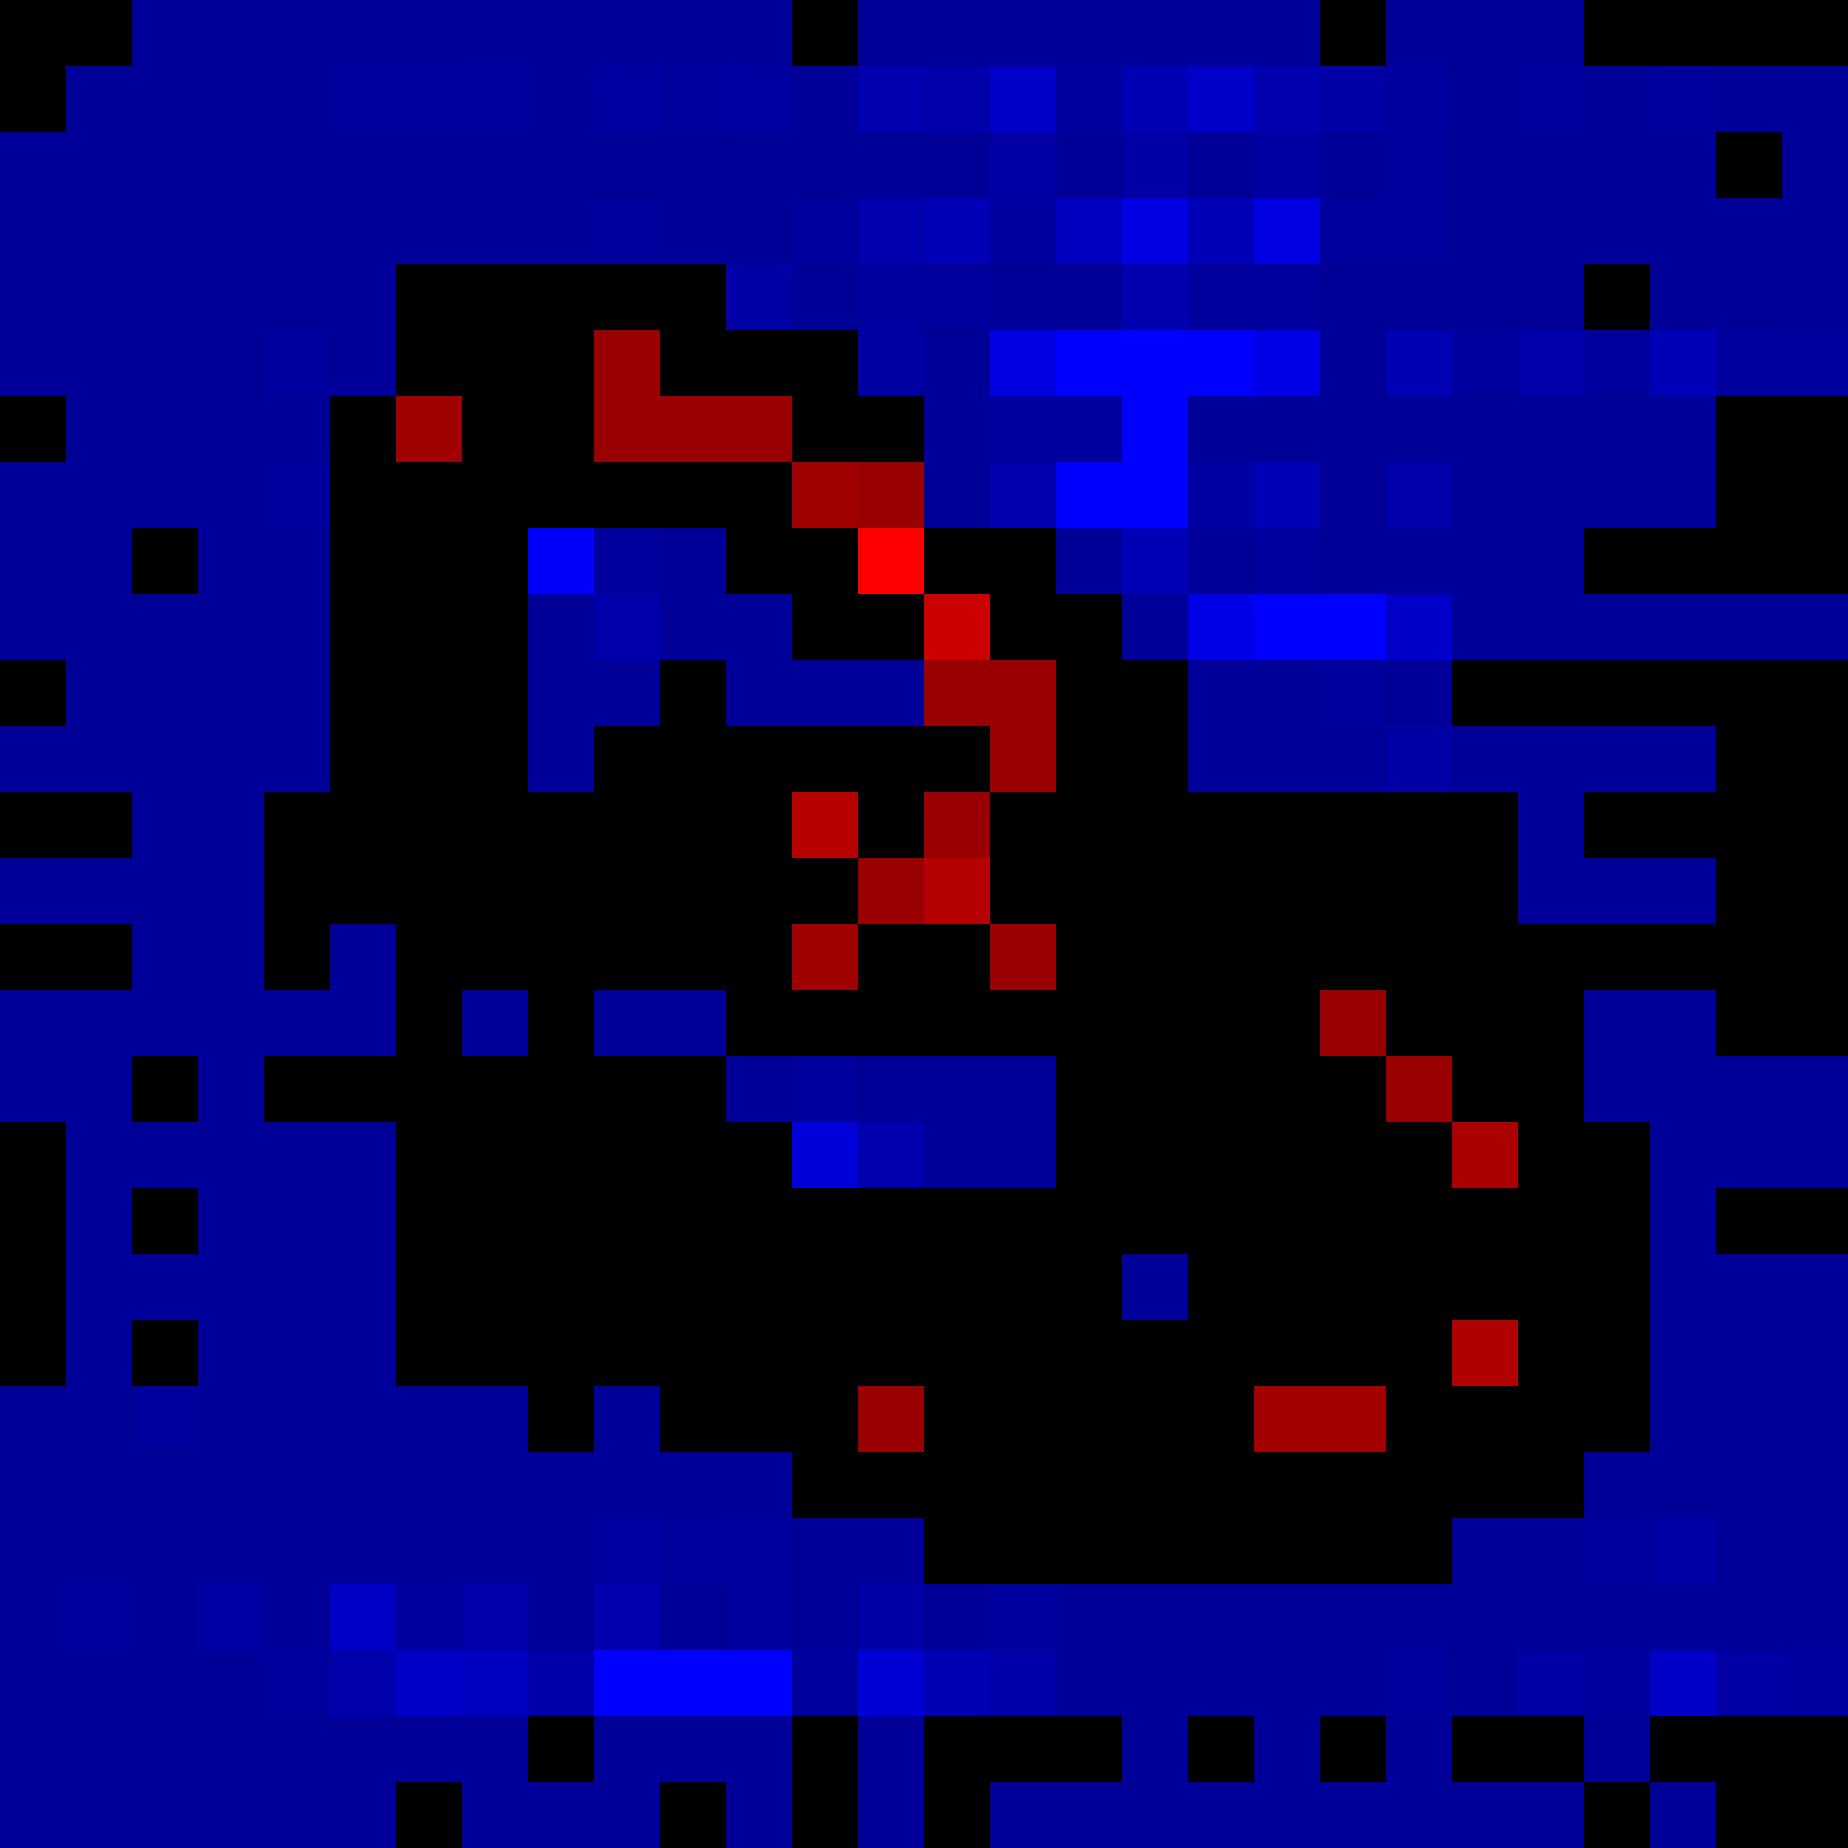
\includegraphics[width=\linewidth]{figures/mnist_split_ic_saliency/image_030_true_3_pred_3/final_saliency_threshold_wrt_3_bright.png}\\[-2pt]{\scriptsize Logit 3}
      \end{minipage}%
      \begin{minipage}[b]{0.19\linewidth}\centering
        
\includegraphics[width=\linewidth]{figures/mnist_split_ic_saliency/image_030_true_3_pred_3/final_saliency_threshold_wrt_4_bright.png}\\[-2pt]{\scriptsize Logit 4}
      \end{minipage}
  
      \vspace{0.12cm}
  
      % Row 2: logits 5..9
      \begin{minipage}[b]{0.19\linewidth}\centering
        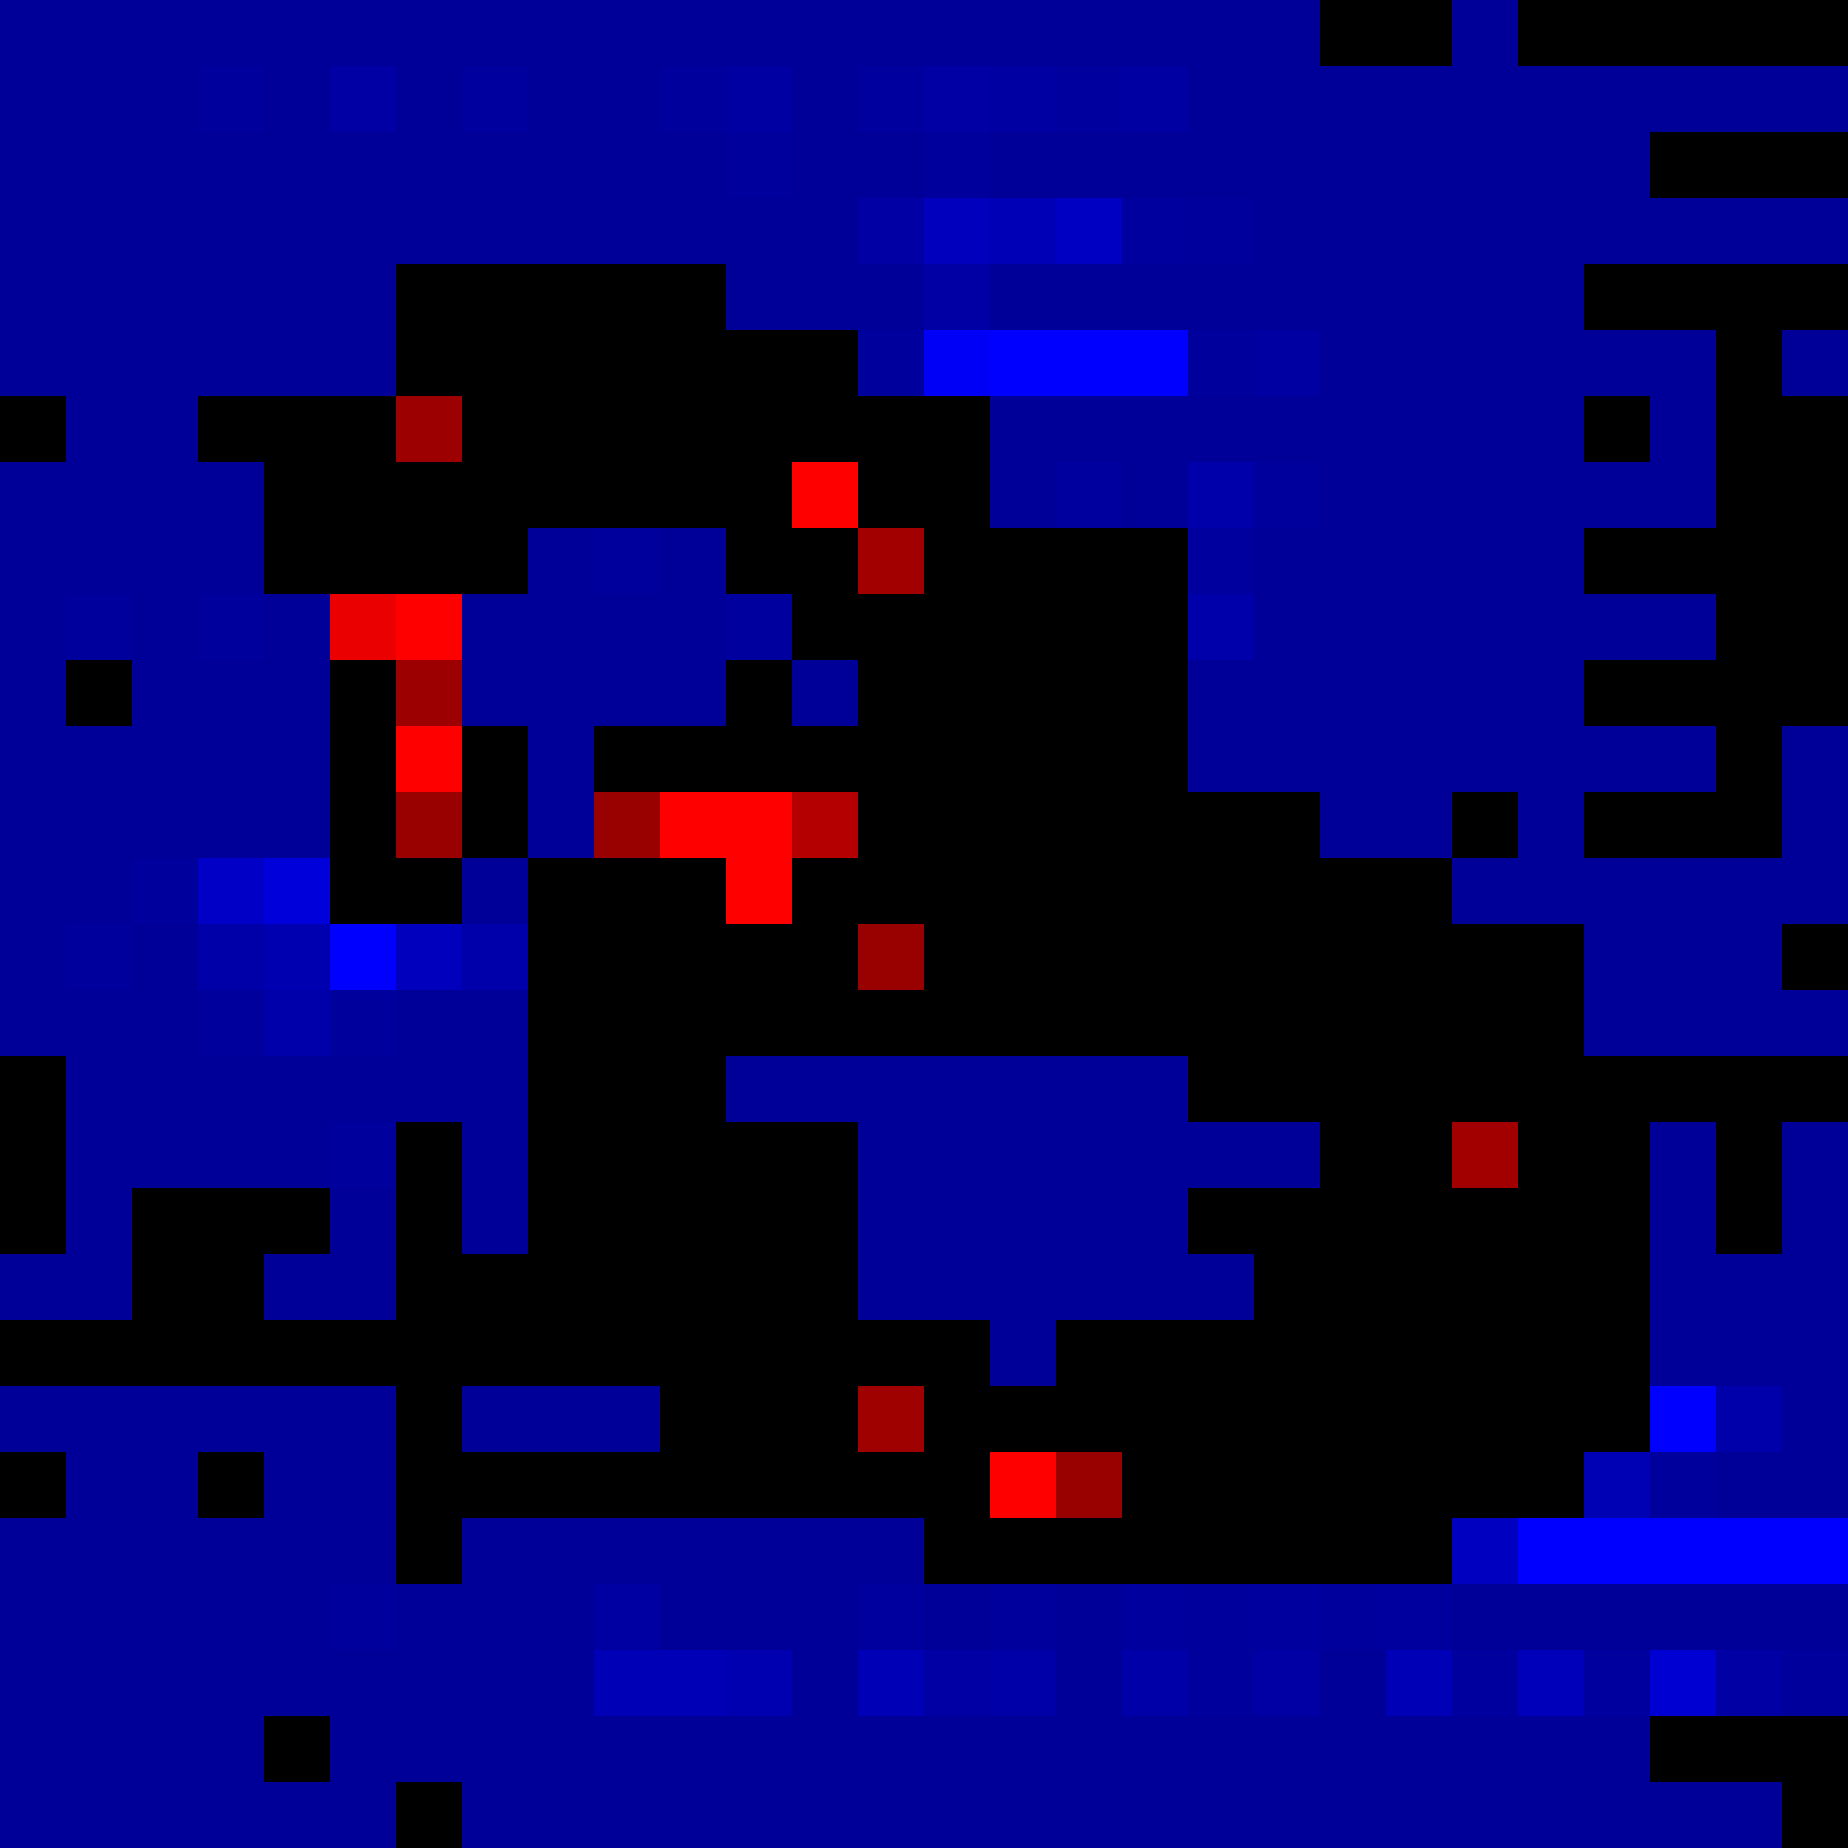
\includegraphics[width=\linewidth]{figures/mnist_split_ic_saliency/image_030_true_3_pred_3/final_saliency_threshold_wrt_5_bright.png}\\[-2pt]{\scriptsize Logit 5}
      \end{minipage}%
      \begin{minipage}[b]{0.19\linewidth}\centering
        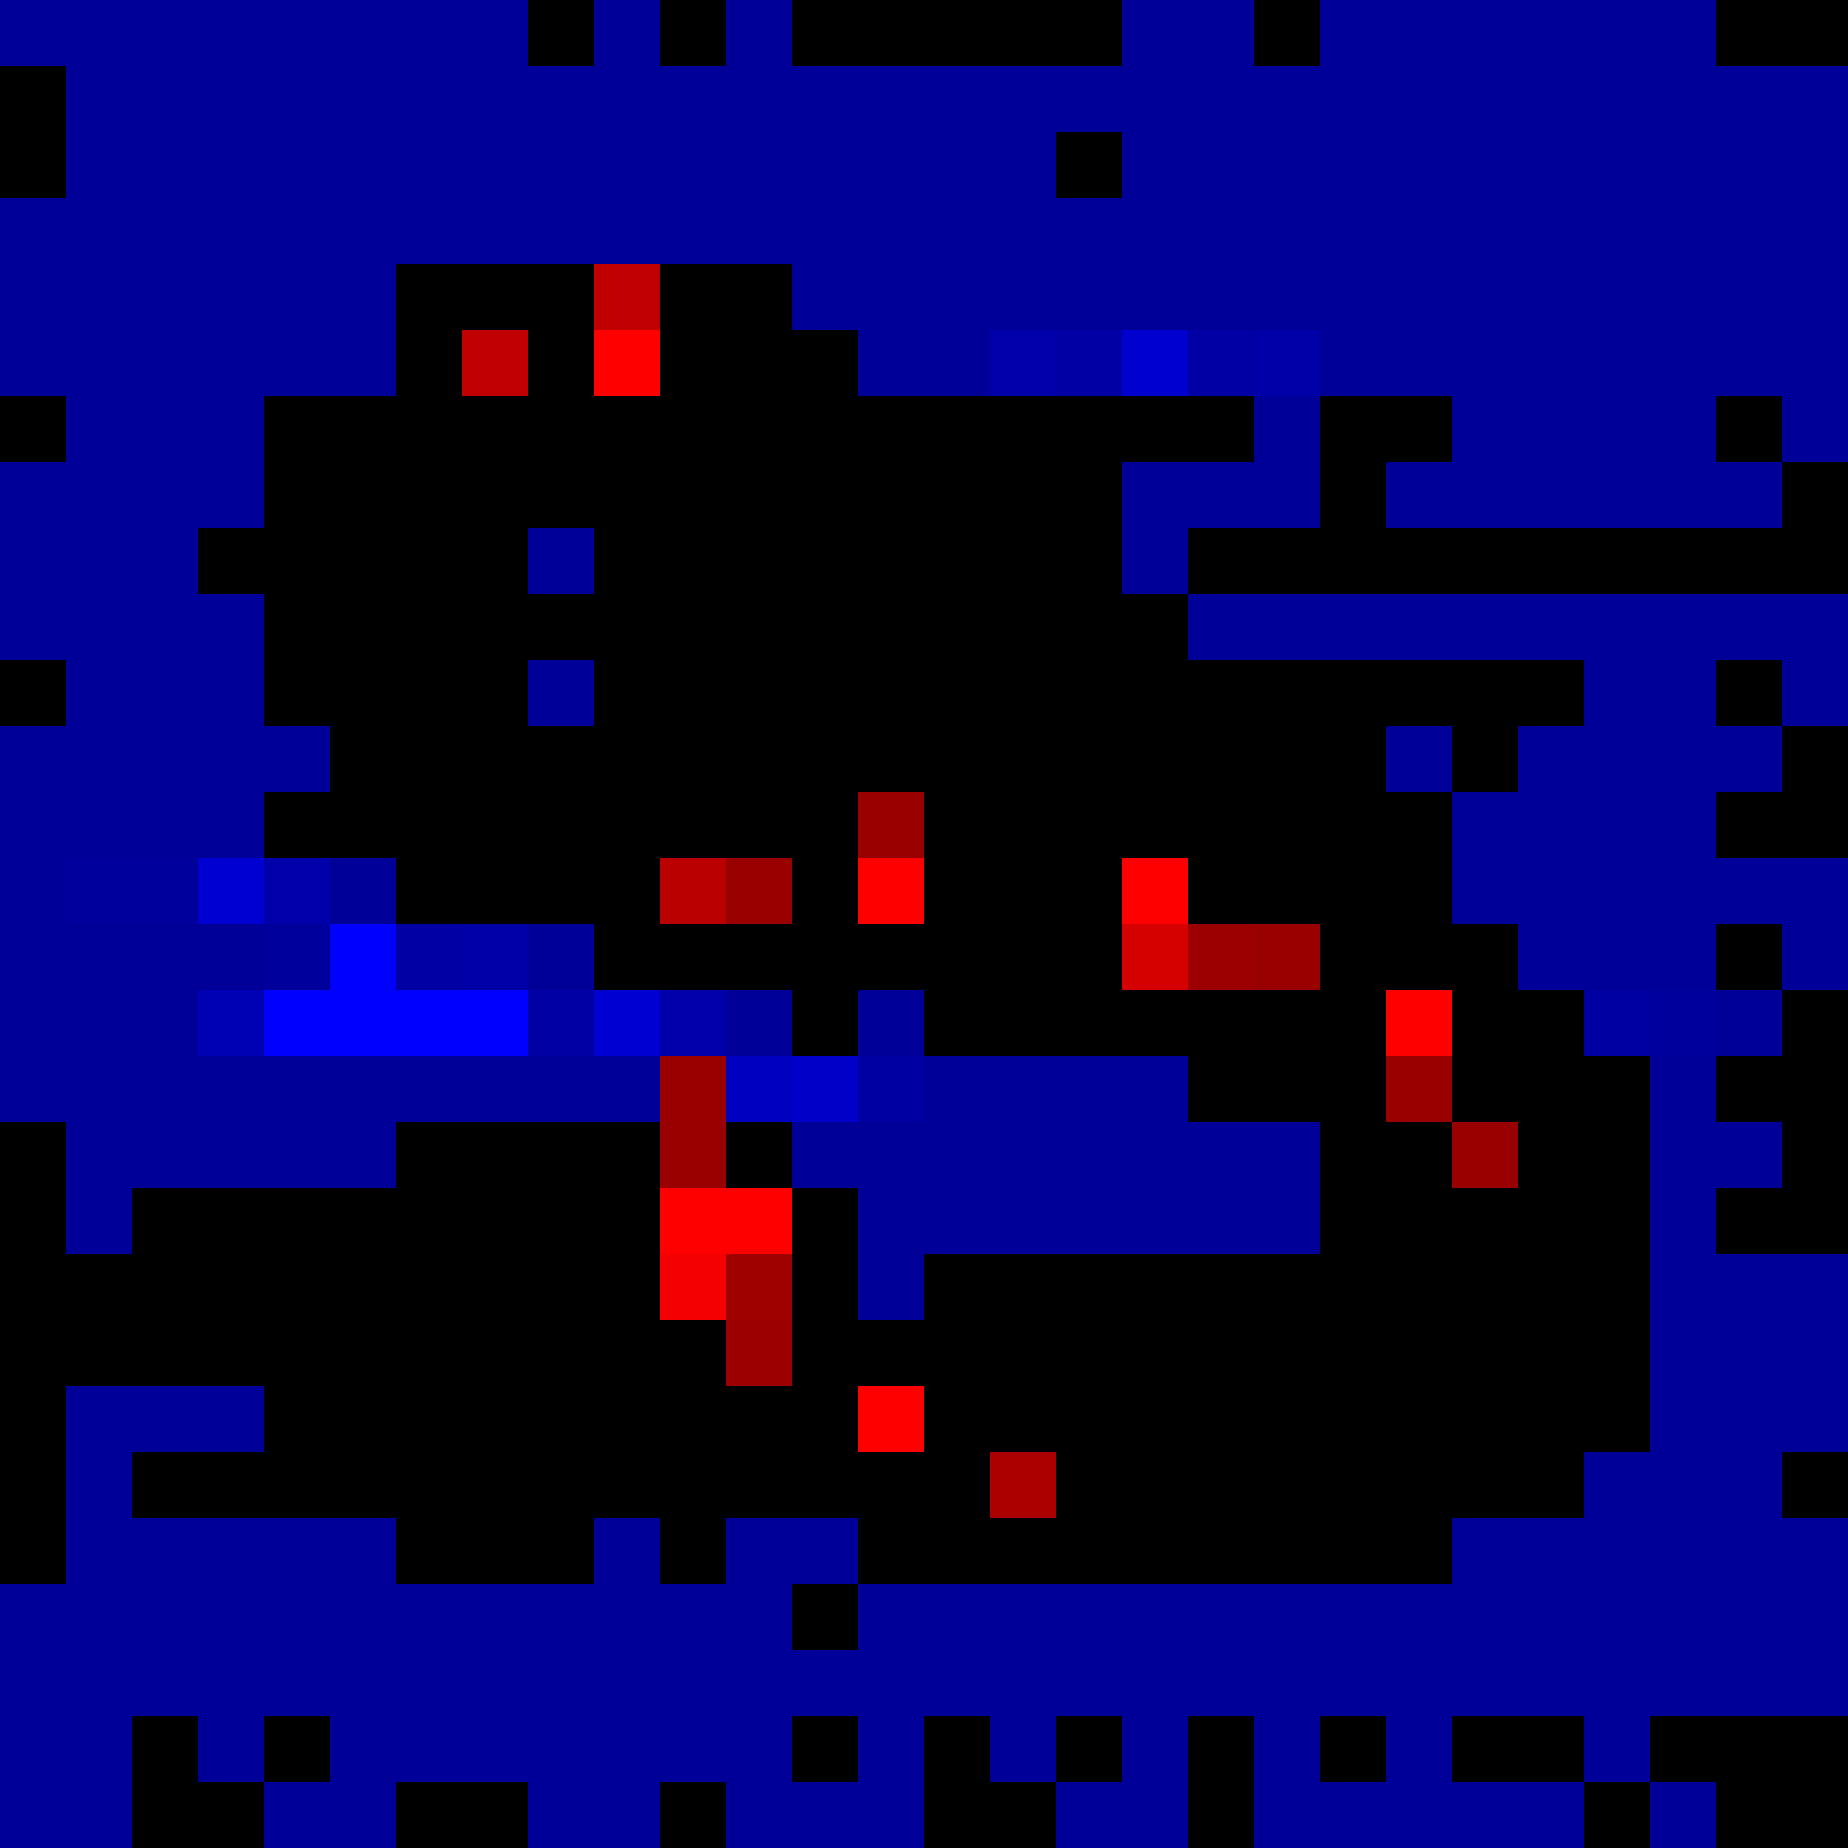
\includegraphics[width=\linewidth]{figures/mnist_split_ic_saliency/image_030_true_3_pred_3/final_saliency_threshold_wrt_6_bright.png}\\[-2pt]{\scriptsize Logit 6}
      \end{minipage}%
      \begin{minipage}[b]{0.19\linewidth}\centering
        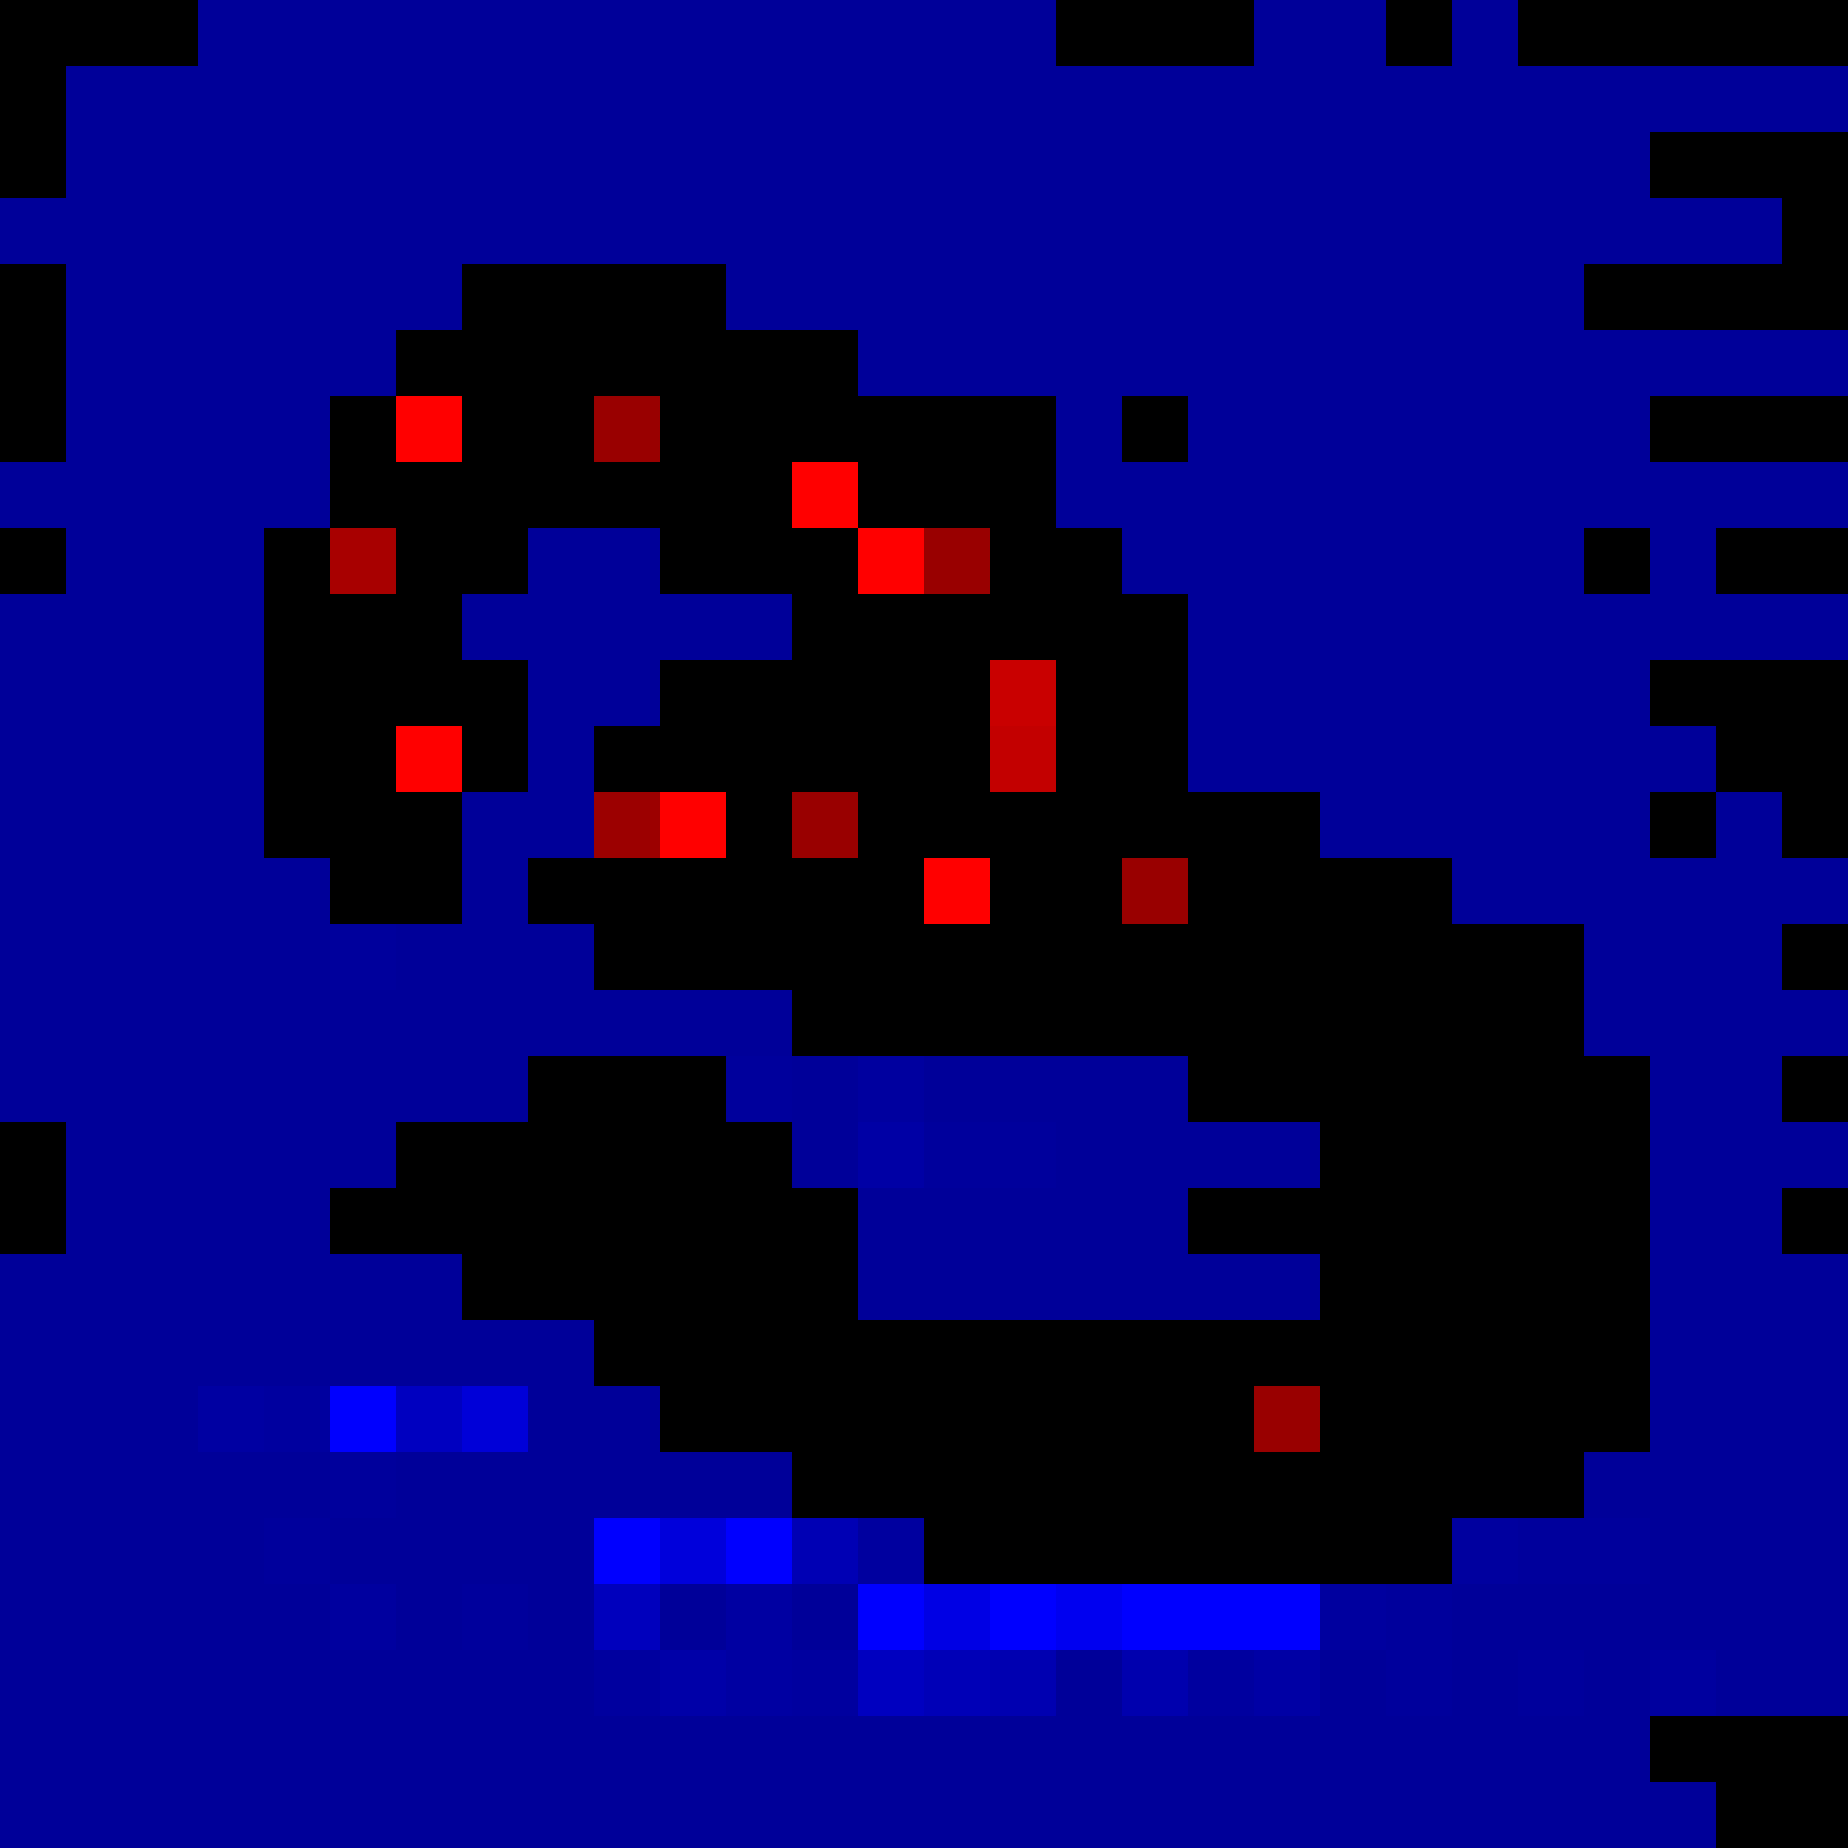
\includegraphics[width=\linewidth]{figures/mnist_split_ic_saliency/image_030_true_3_pred_3/final_saliency_threshold_wrt_7_bright.png}\\[-2pt]{\scriptsize Logit 7}
      \end{minipage}%
      \begin{minipage}[b]{0.19\linewidth}\centering
        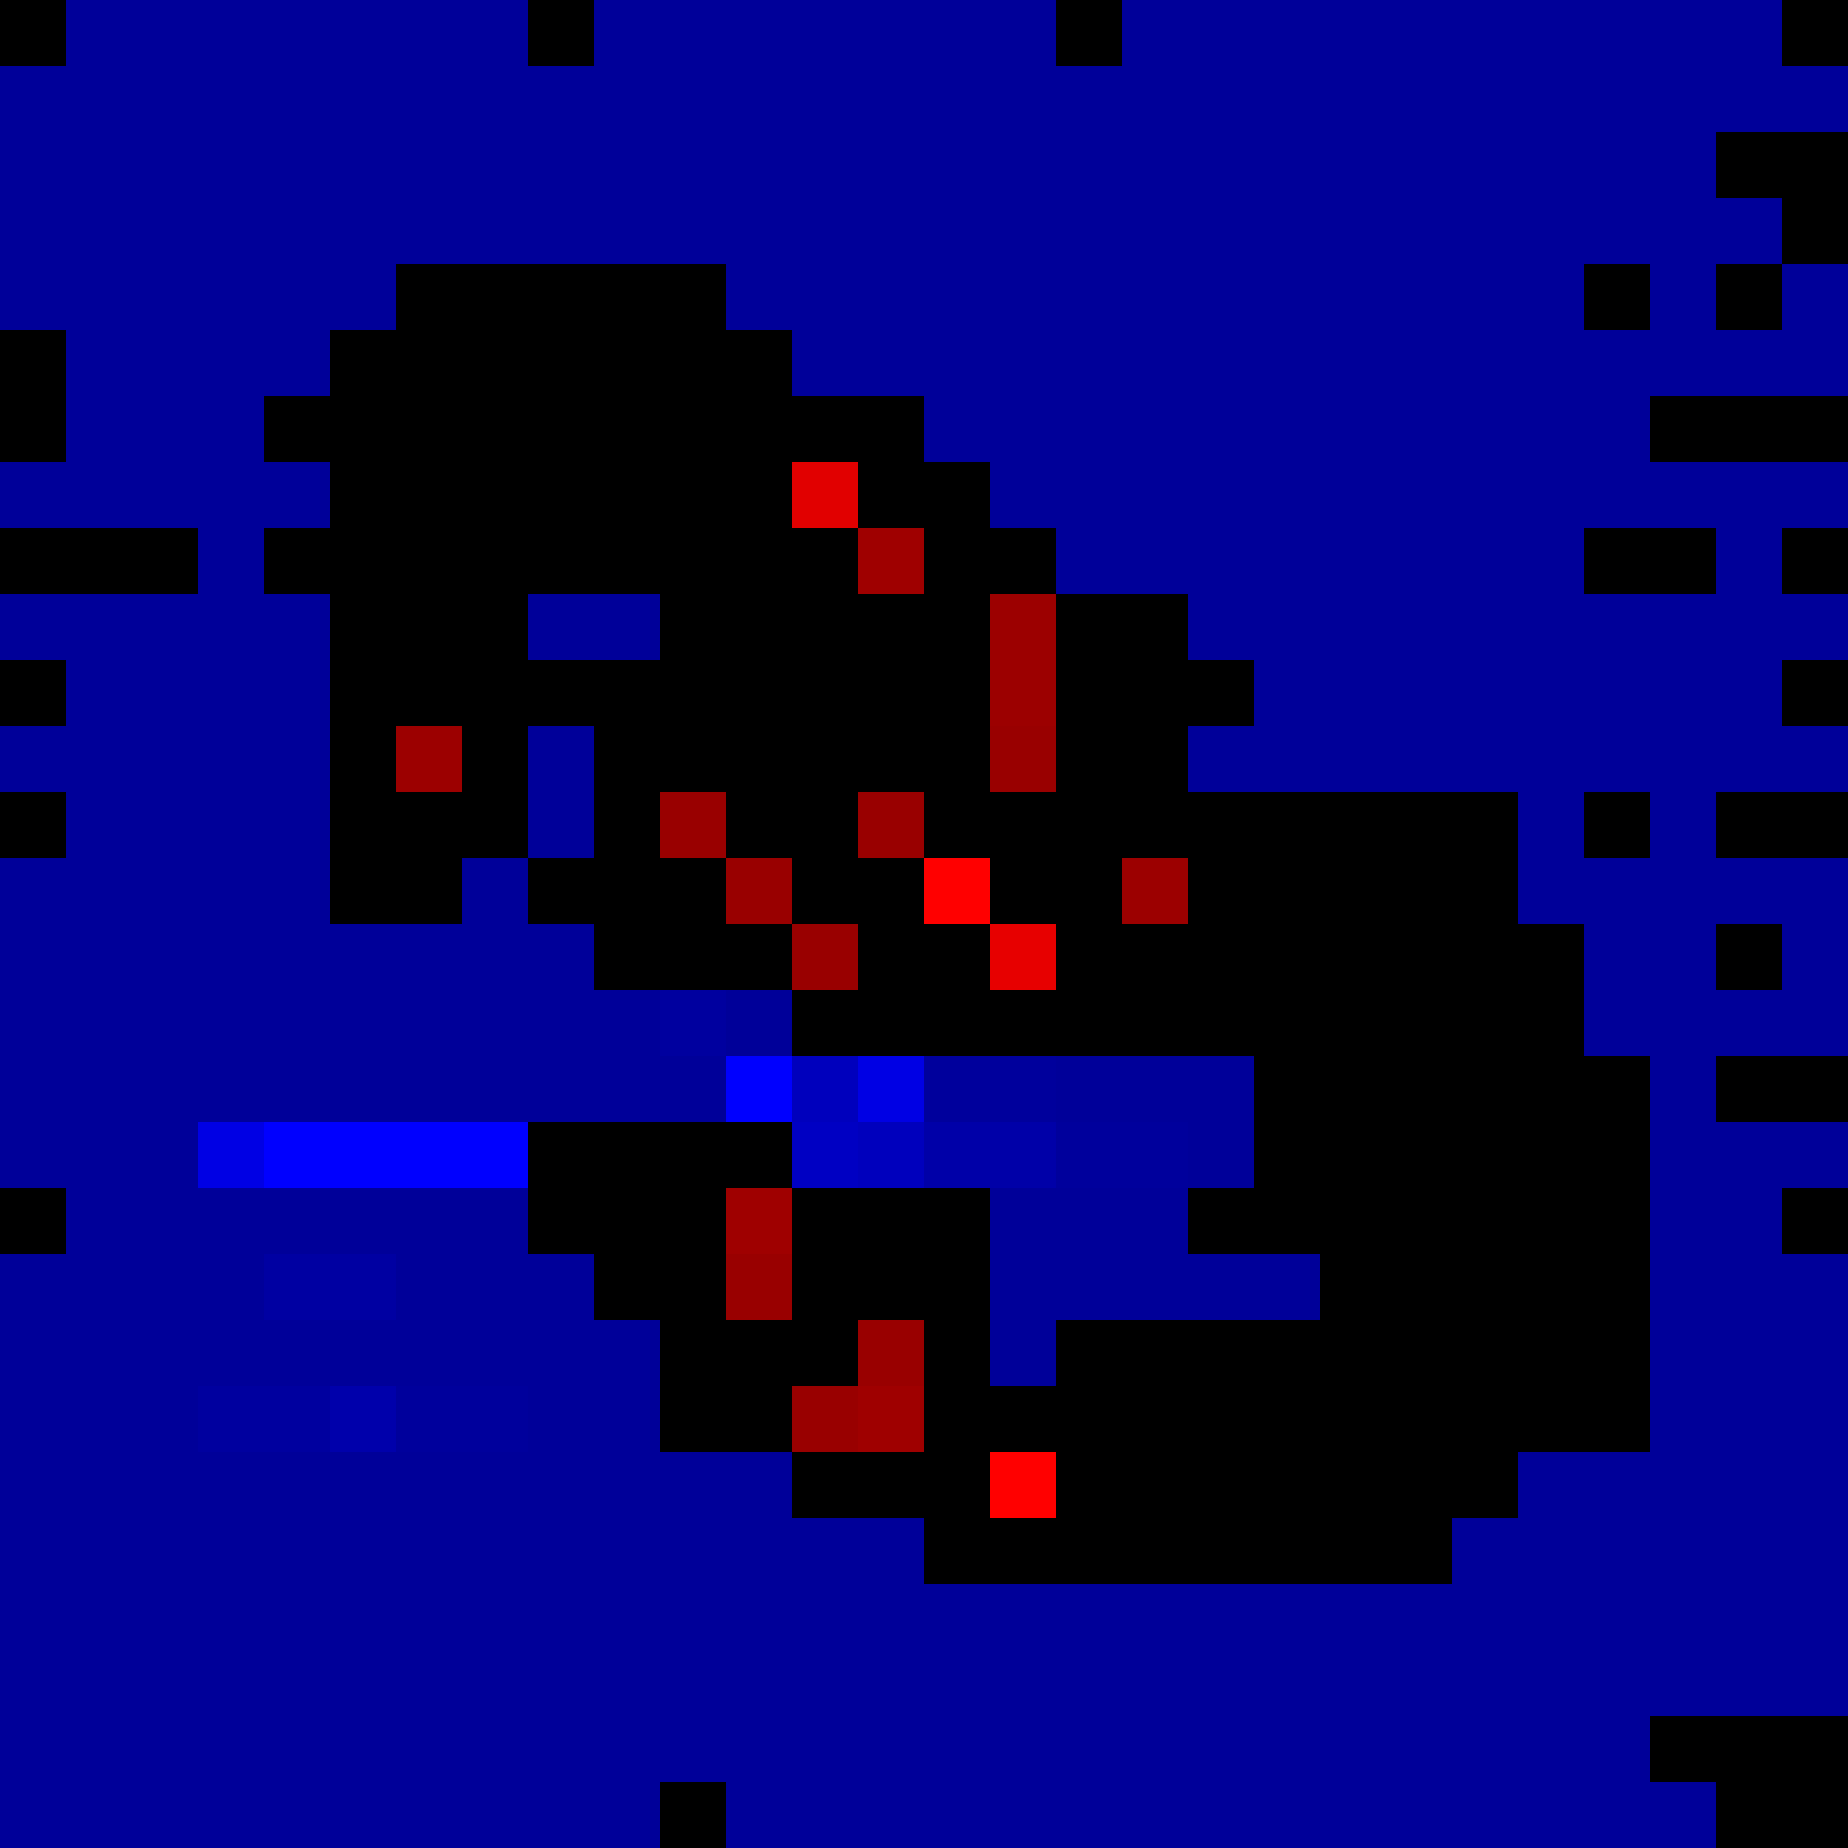
\includegraphics[width=\linewidth]{figures/mnist_split_ic_saliency/image_030_true_3_pred_3/final_saliency_threshold_wrt_8_bright.png}\\[-2pt]{\scriptsize Logit 8}
      \end{minipage}%
      \begin{minipage}[b]{0.19\linewidth}\centering
        
\includegraphics[width=\linewidth]{figures/mnist_split_ic_saliency/image_030_true_3_pred_3/final_saliency_threshold_wrt_9_bright.png}\\[-2pt]{\scriptsize Logit 9}
      \end{minipage}
    \end{minipage}
  
    \vspace{0.35cm}
  
    %------------------ Example B: image_036 ------------------
    \begin{minipage}[c]{0.16\linewidth}
      \centering
      
\includegraphics[width=\linewidth]{figures/mnist_split_ic_saliency/image_036_true_3_pred_3/original.png}\\[-2pt]
      {\scriptsize Original}
    \end{minipage}\hspace{0.01\linewidth}%
    \begin{minipage}[c]{0.81\linewidth}
      \centering
      % Row 1: logits 0..4
      \begin{minipage}[b]{0.19\linewidth}\centering
        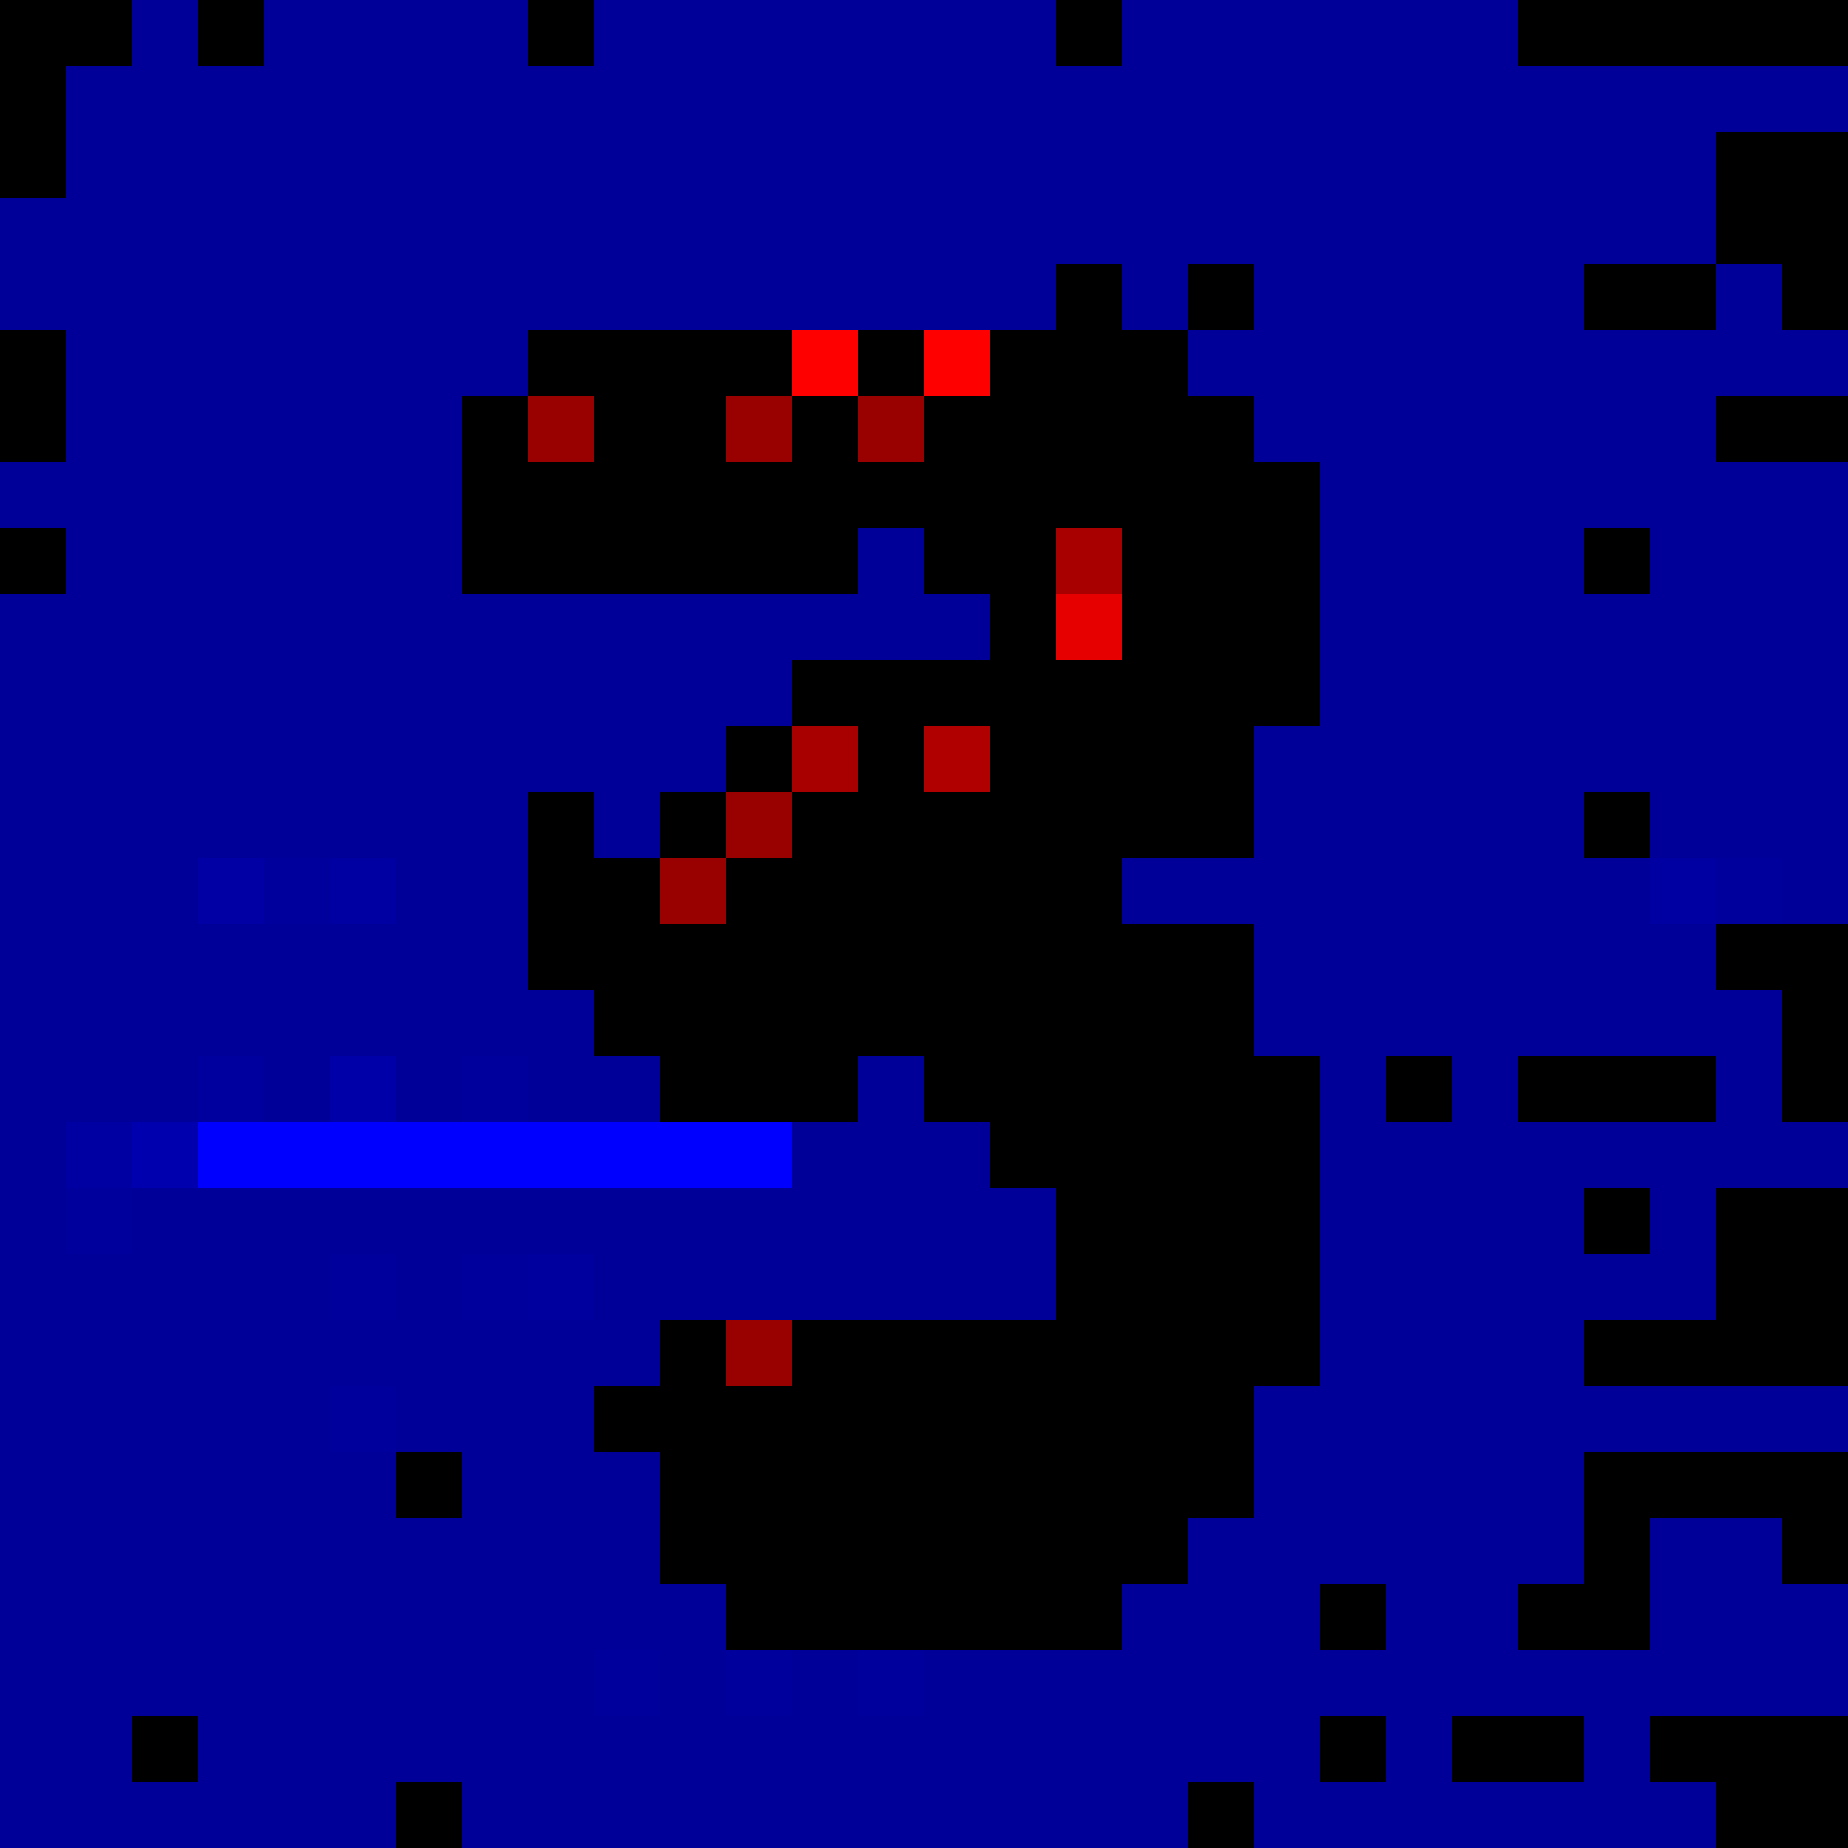
\includegraphics[width=\linewidth]{figures/mnist_split_ic_saliency/image_036_true_3_pred_3/final_saliency_threshold_wrt_0_bright.png}\\[-2pt]{\scriptsize Logit 0}
      \end{minipage}%
      \begin{minipage}[b]{0.19\linewidth}\centering
        
\includegraphics[width=\linewidth]{figures/mnist_split_ic_saliency/image_036_true_3_pred_3/final_saliency_threshold_wrt_1_bright.png}\\[-2pt]{\scriptsize Logit 1}
      \end{minipage}%
      \begin{minipage}[b]{0.19\linewidth}\centering
        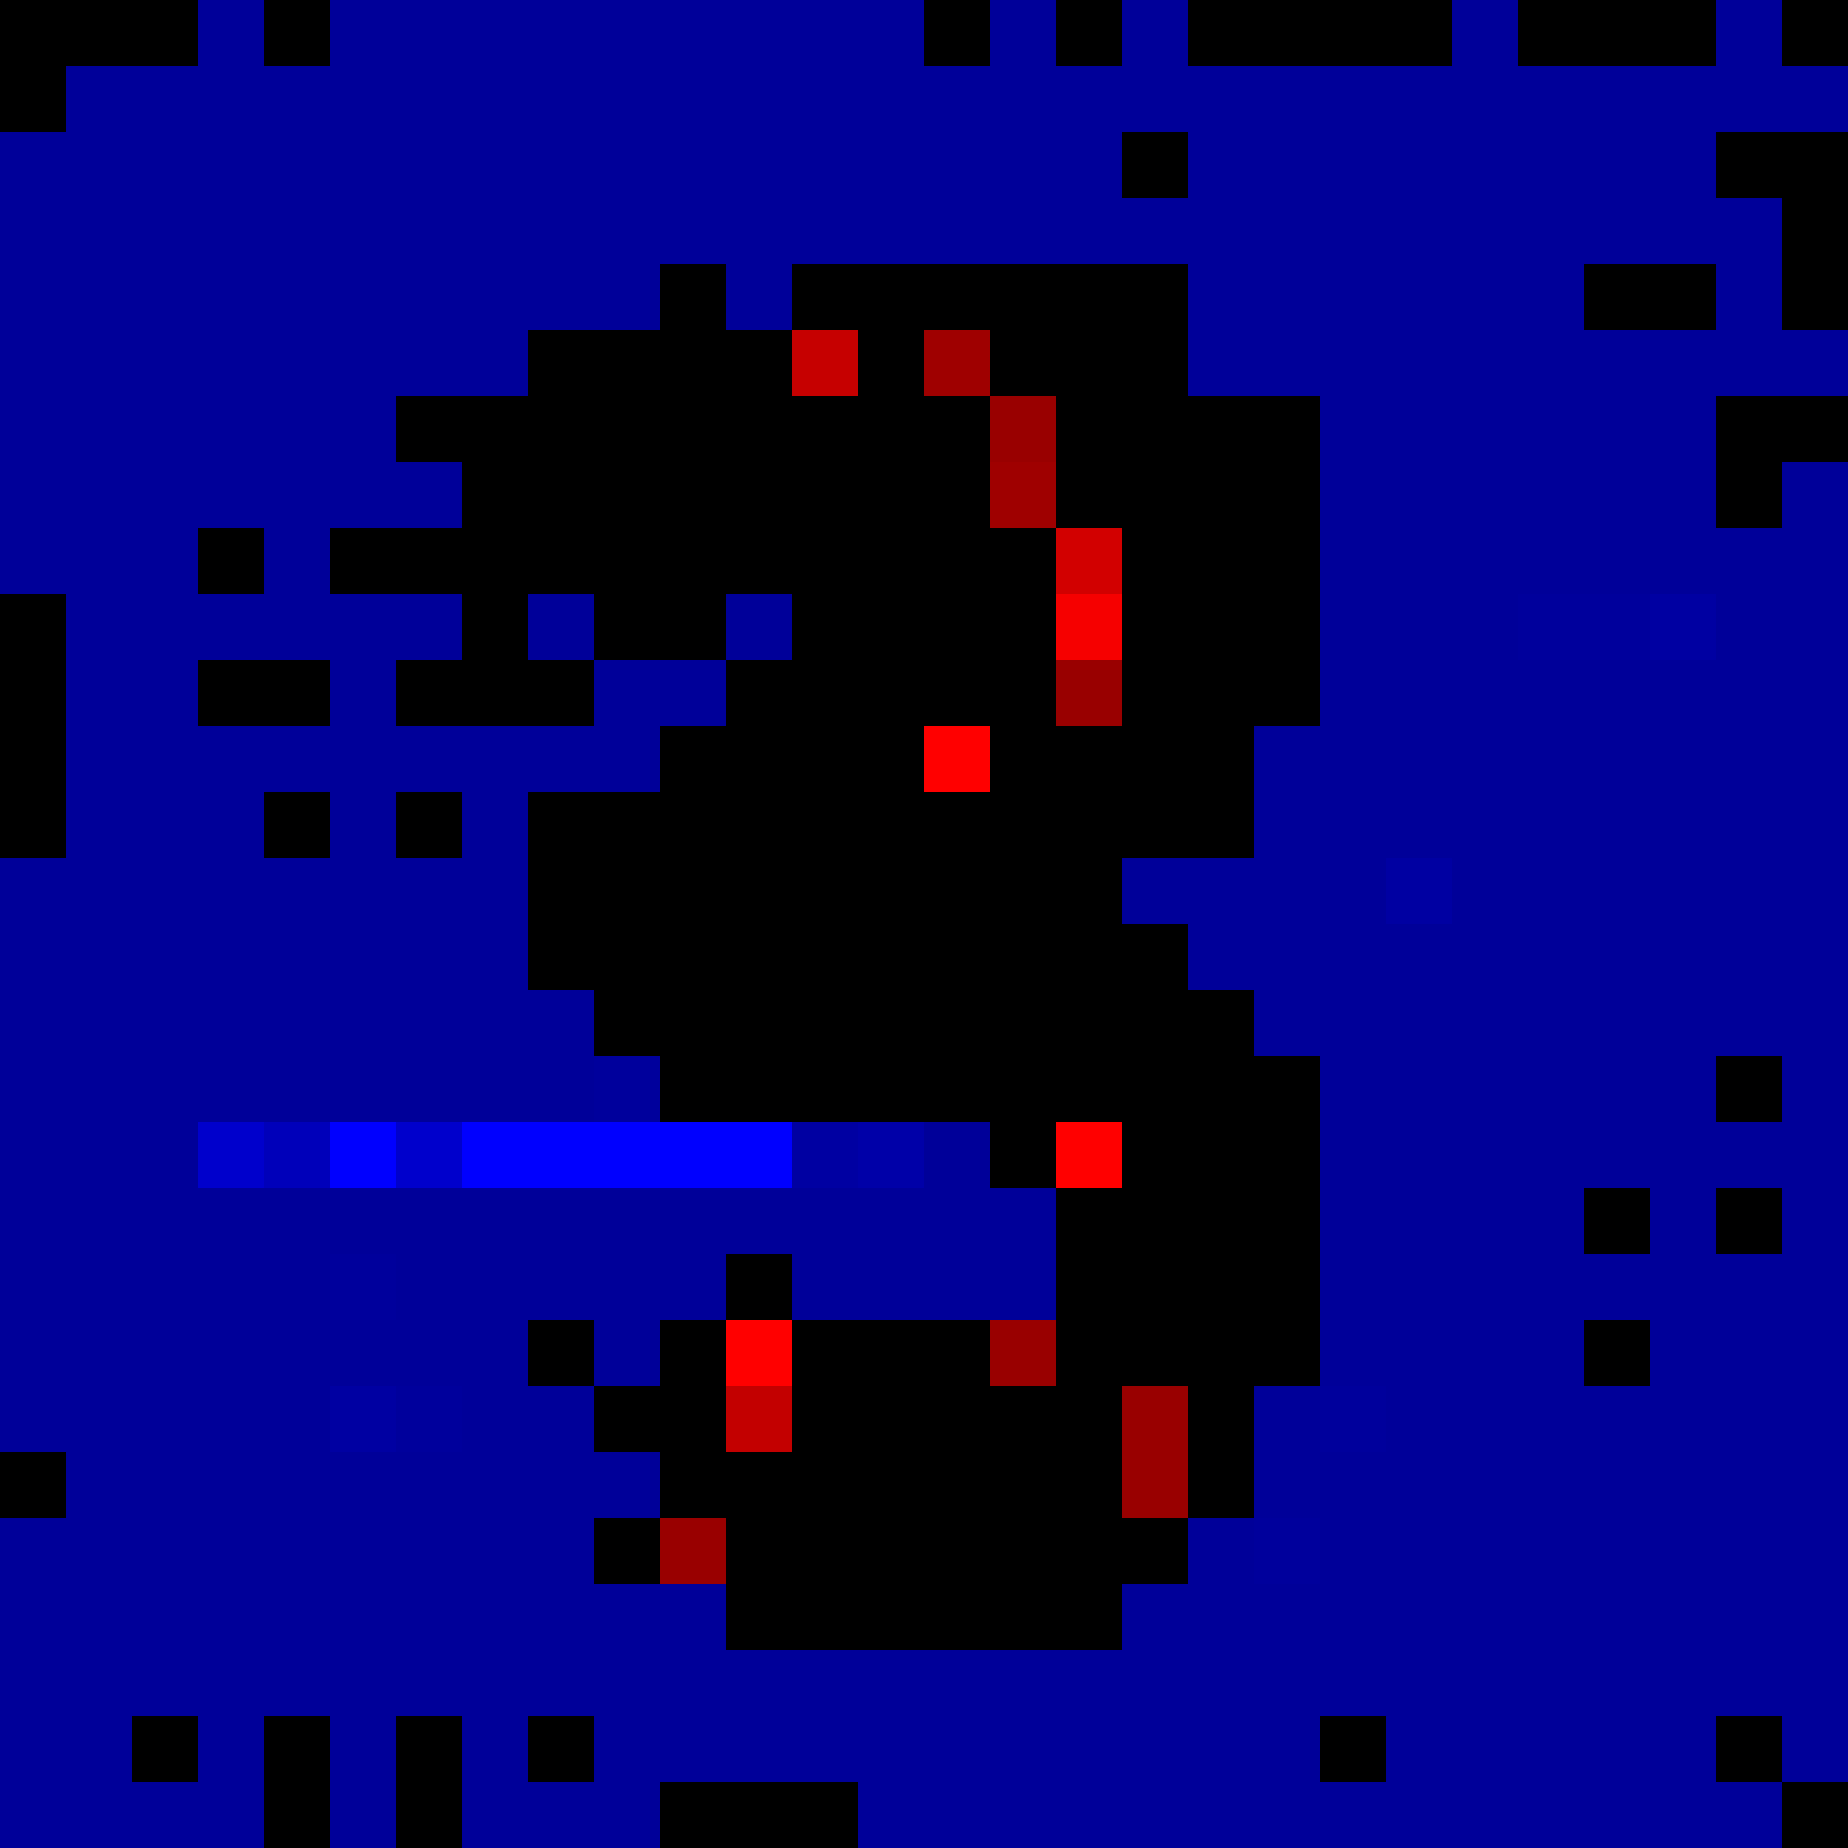
\includegraphics[width=\linewidth]{figures/mnist_split_ic_saliency/image_036_true_3_pred_3/final_saliency_threshold_wrt_2_bright.png}\\[-2pt]{\scriptsize Logit 2}
      \end{minipage}%
      \begin{minipage}[b]{0.19\linewidth}\centering
        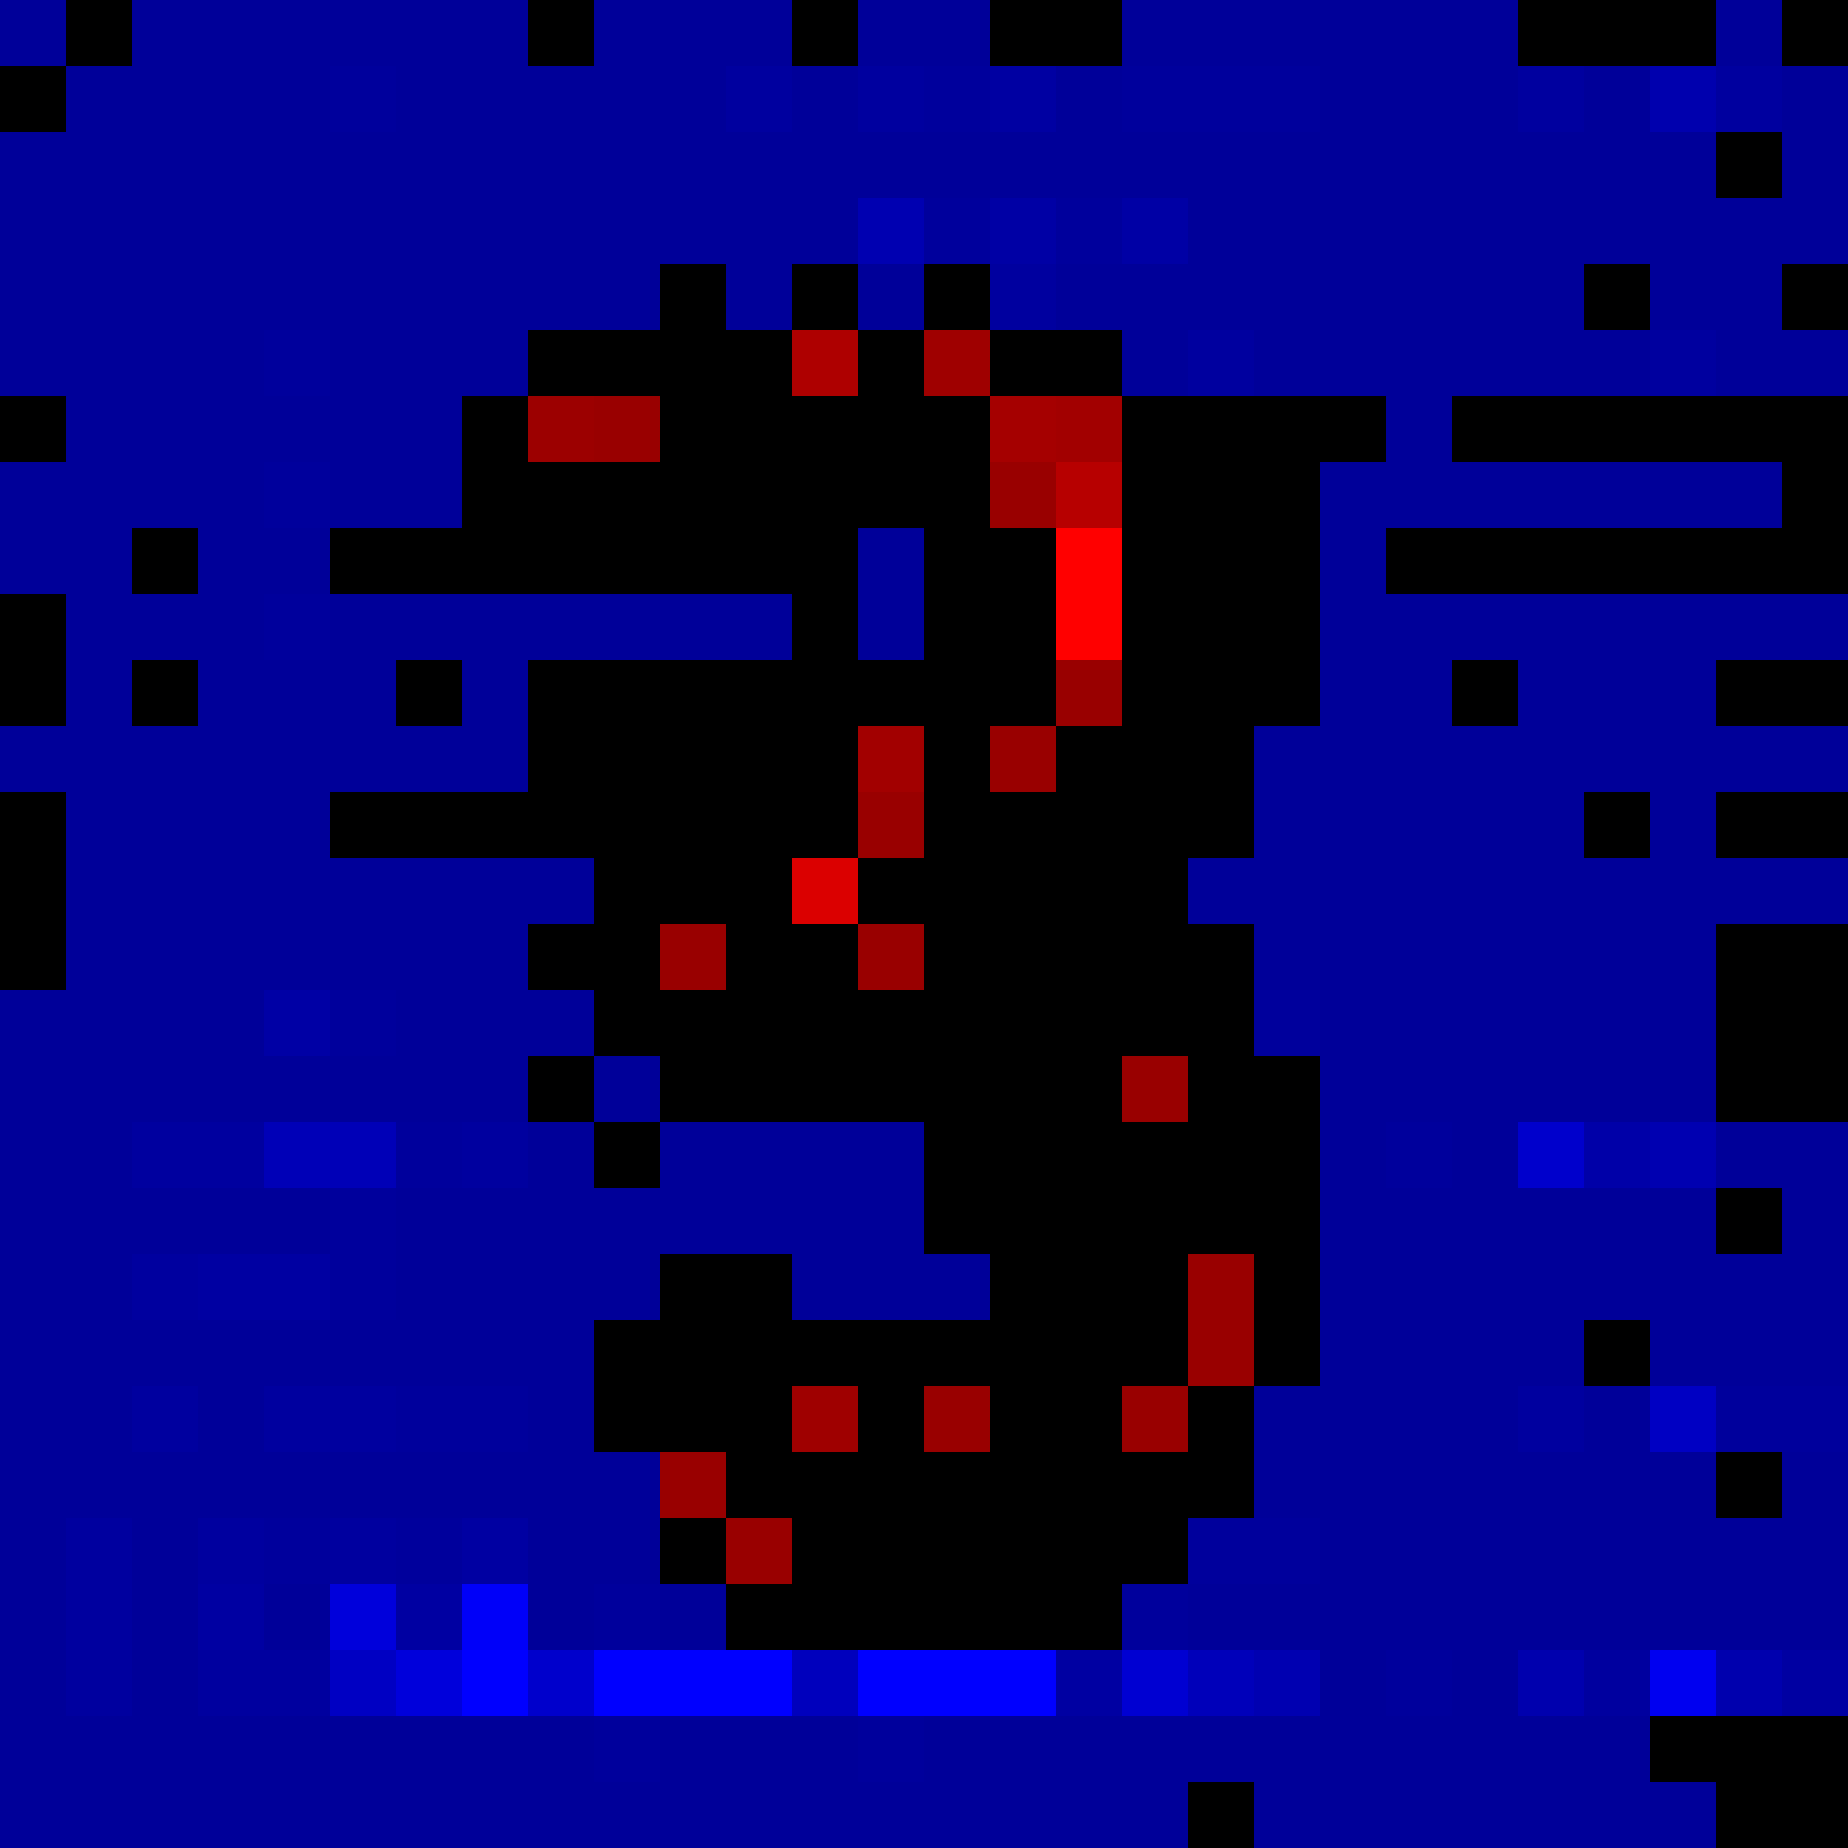
\includegraphics[width=\linewidth]{figures/mnist_split_ic_saliency/image_036_true_3_pred_3/final_saliency_threshold_wrt_3_bright.png}\\[-2pt]{\scriptsize Logit 3}
      \end{minipage}%
      \begin{minipage}[b]{0.19\linewidth}\centering
        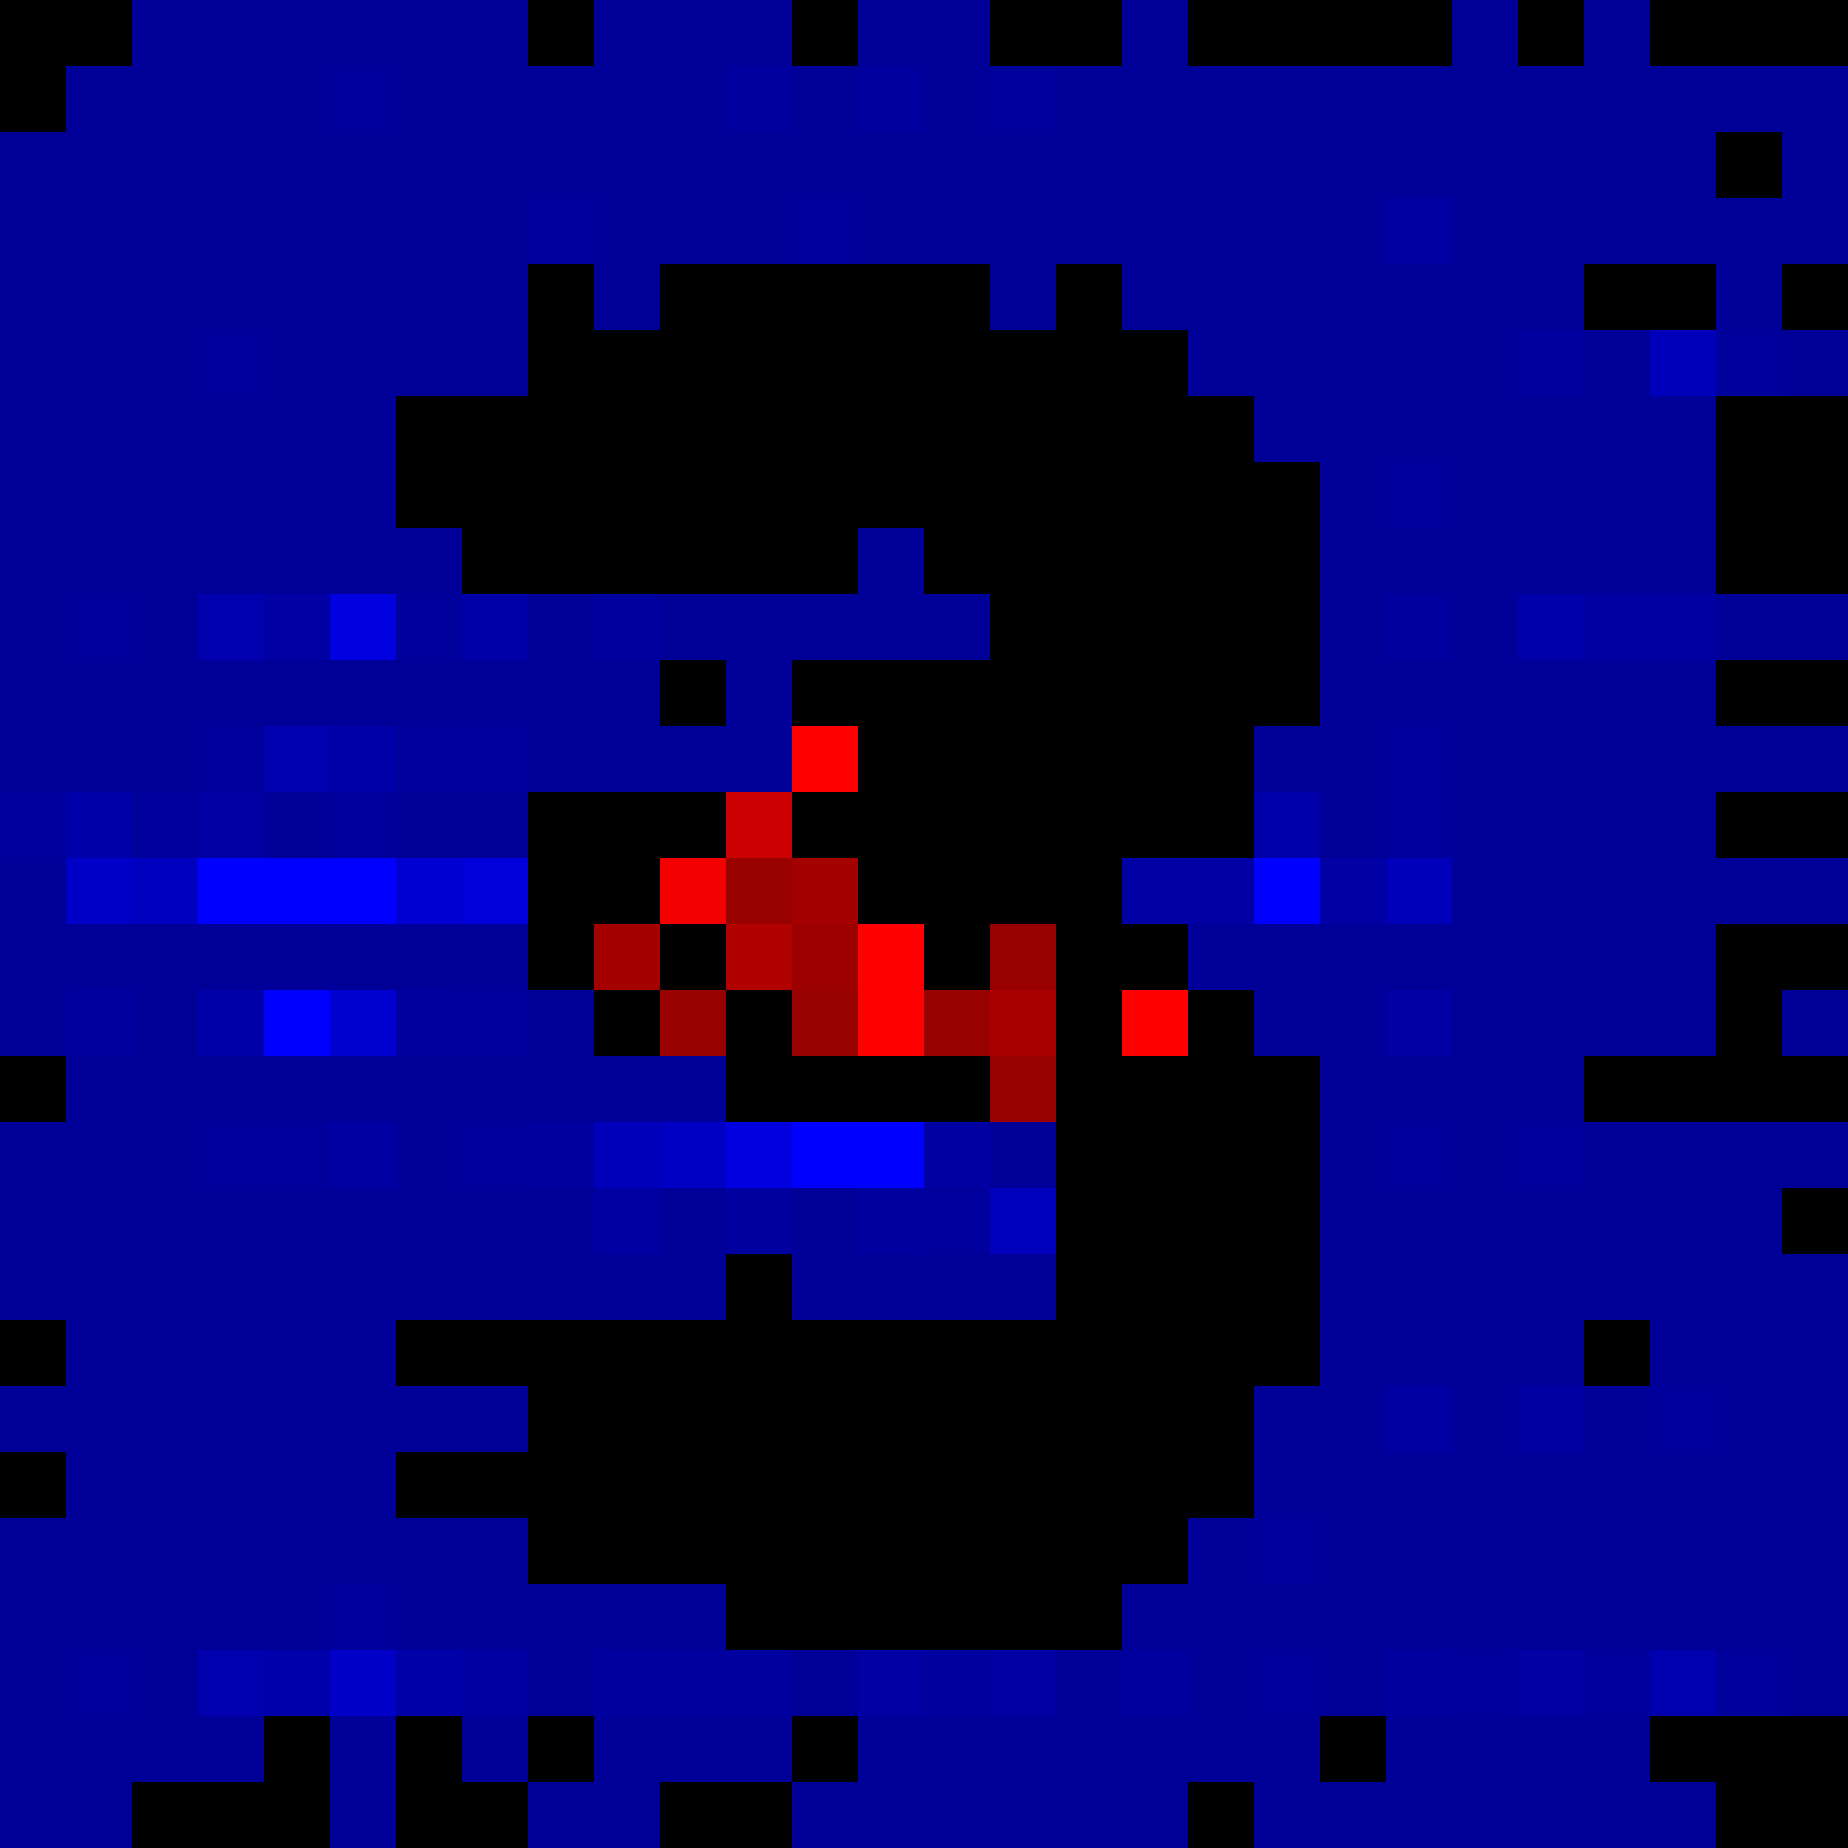
\includegraphics[width=\linewidth]{figures/mnist_split_ic_saliency/image_036_true_3_pred_3/final_saliency_threshold_wrt_4_bright.png}\\[-2pt]{\scriptsize Logit 4}
      \end{minipage}
  
      \vspace{0.12cm}
  
      % Row 2: logits 5..9
      \begin{minipage}[b]{0.19\linewidth}\centering
        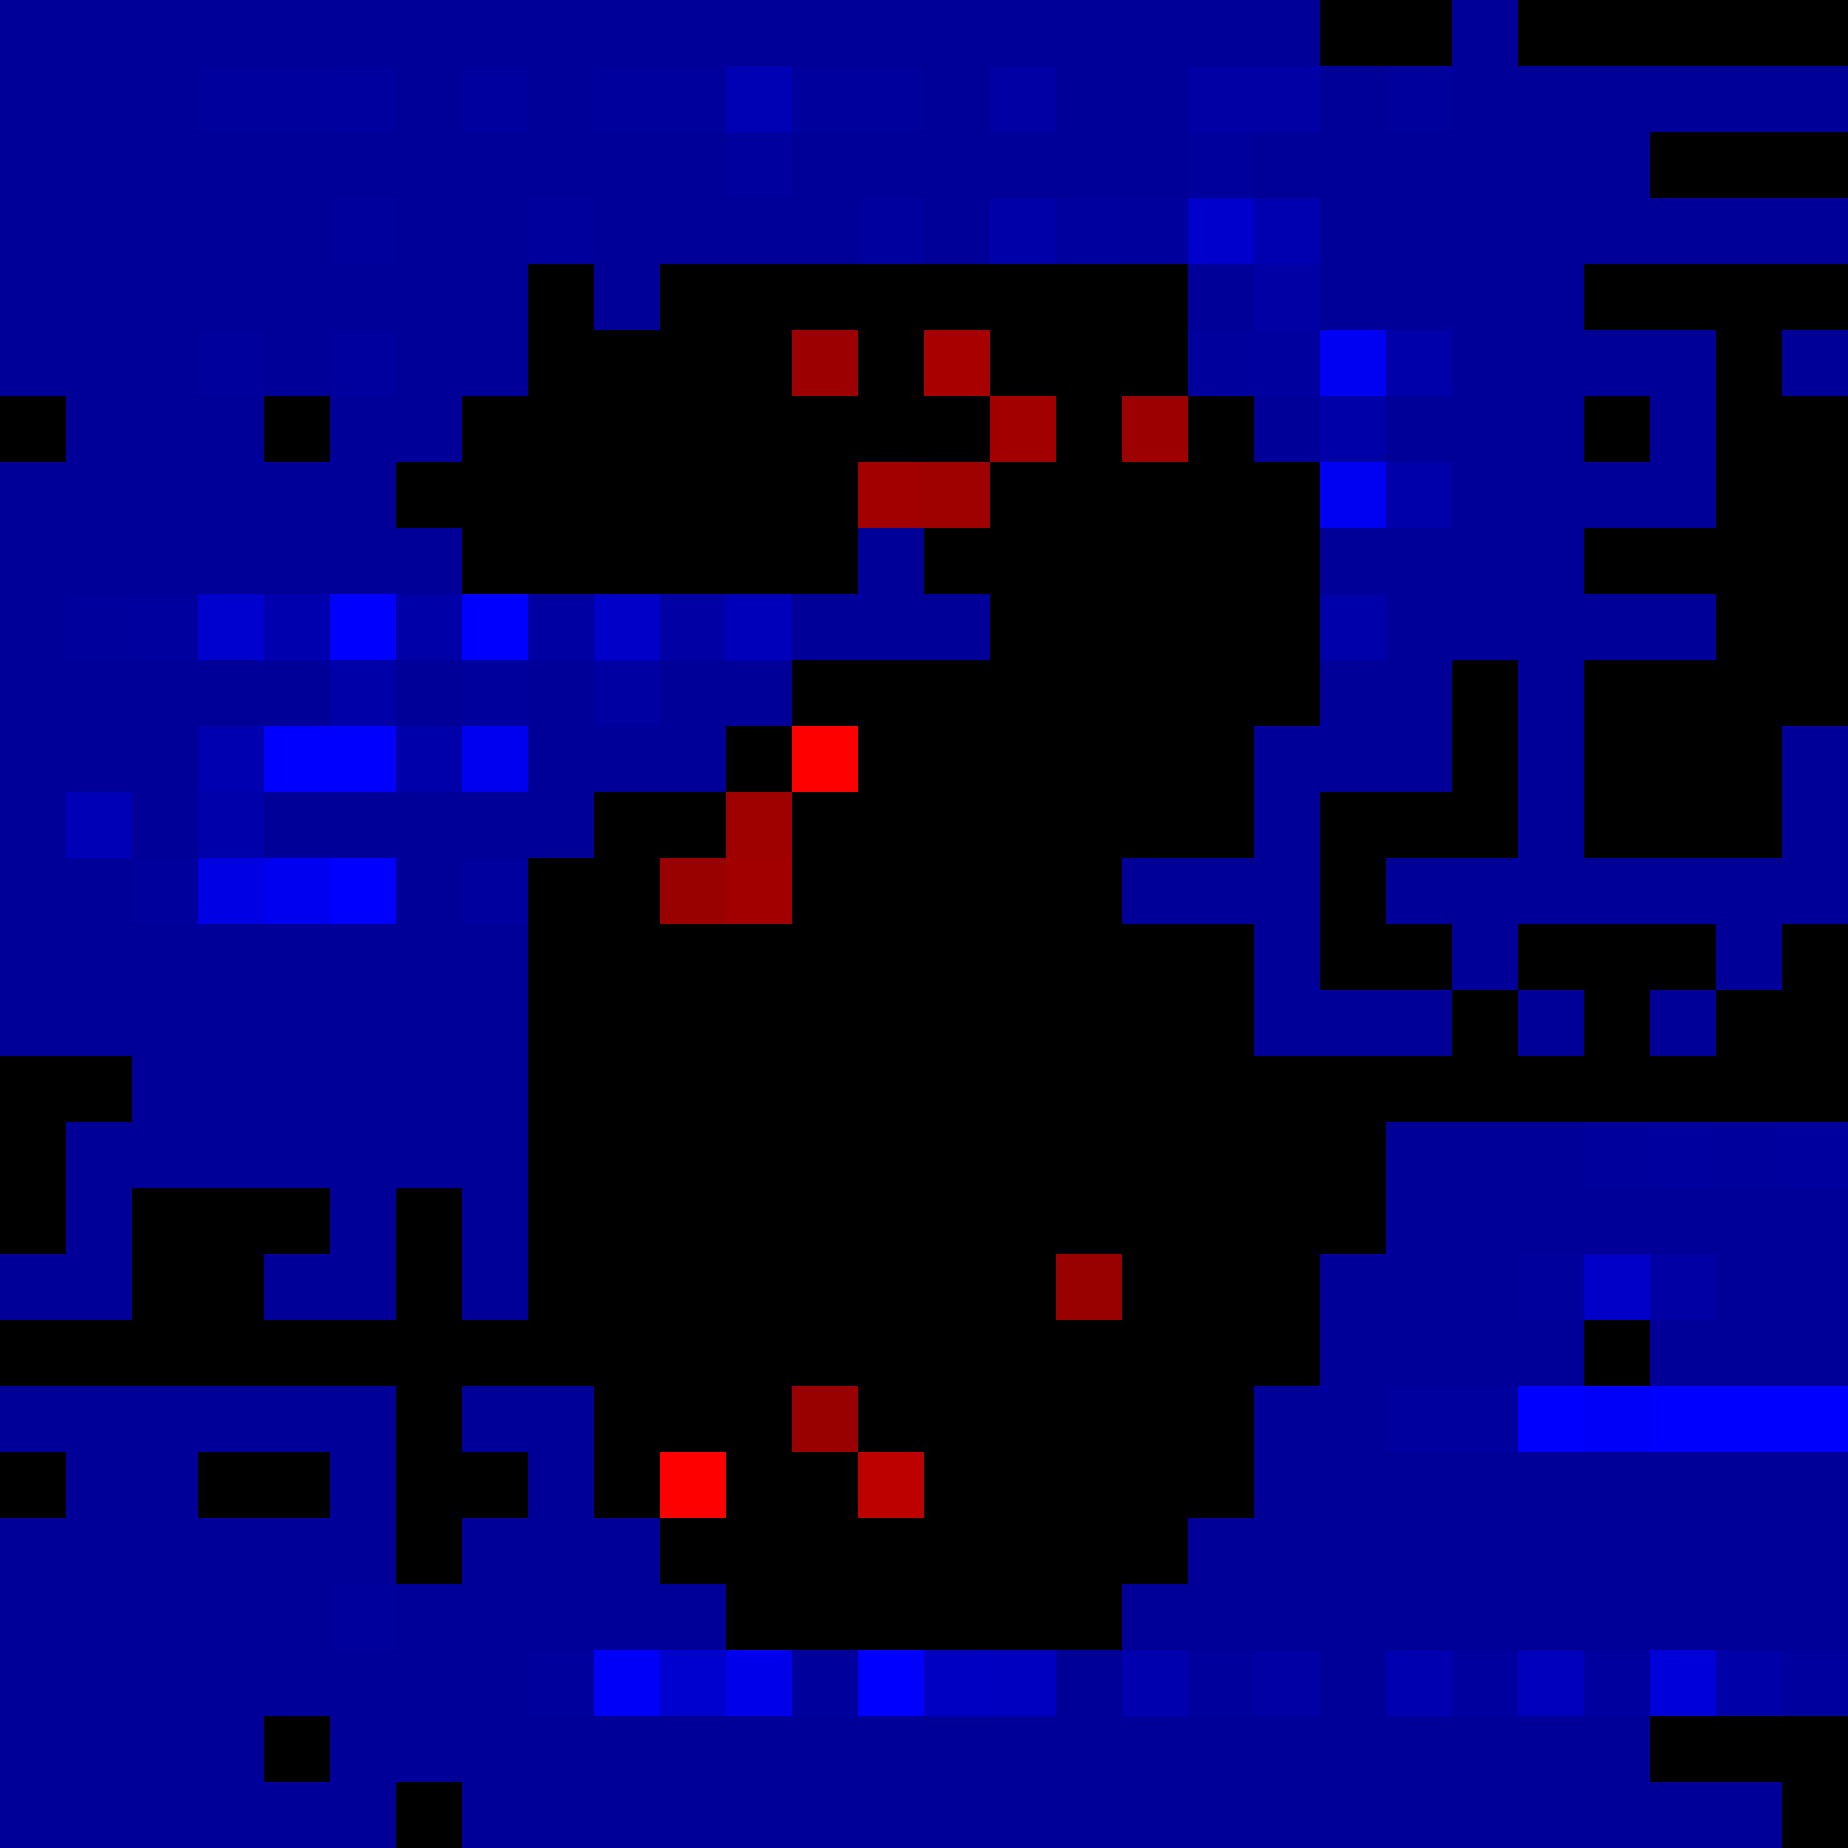
\includegraphics[width=\linewidth]{figures/mnist_split_ic_saliency/image_036_true_3_pred_3/final_saliency_threshold_wrt_5_bright.png}\\[-2pt]{\scriptsize Logit 5}
      \end{minipage}%
      \begin{minipage}[b]{0.19\linewidth}\centering
        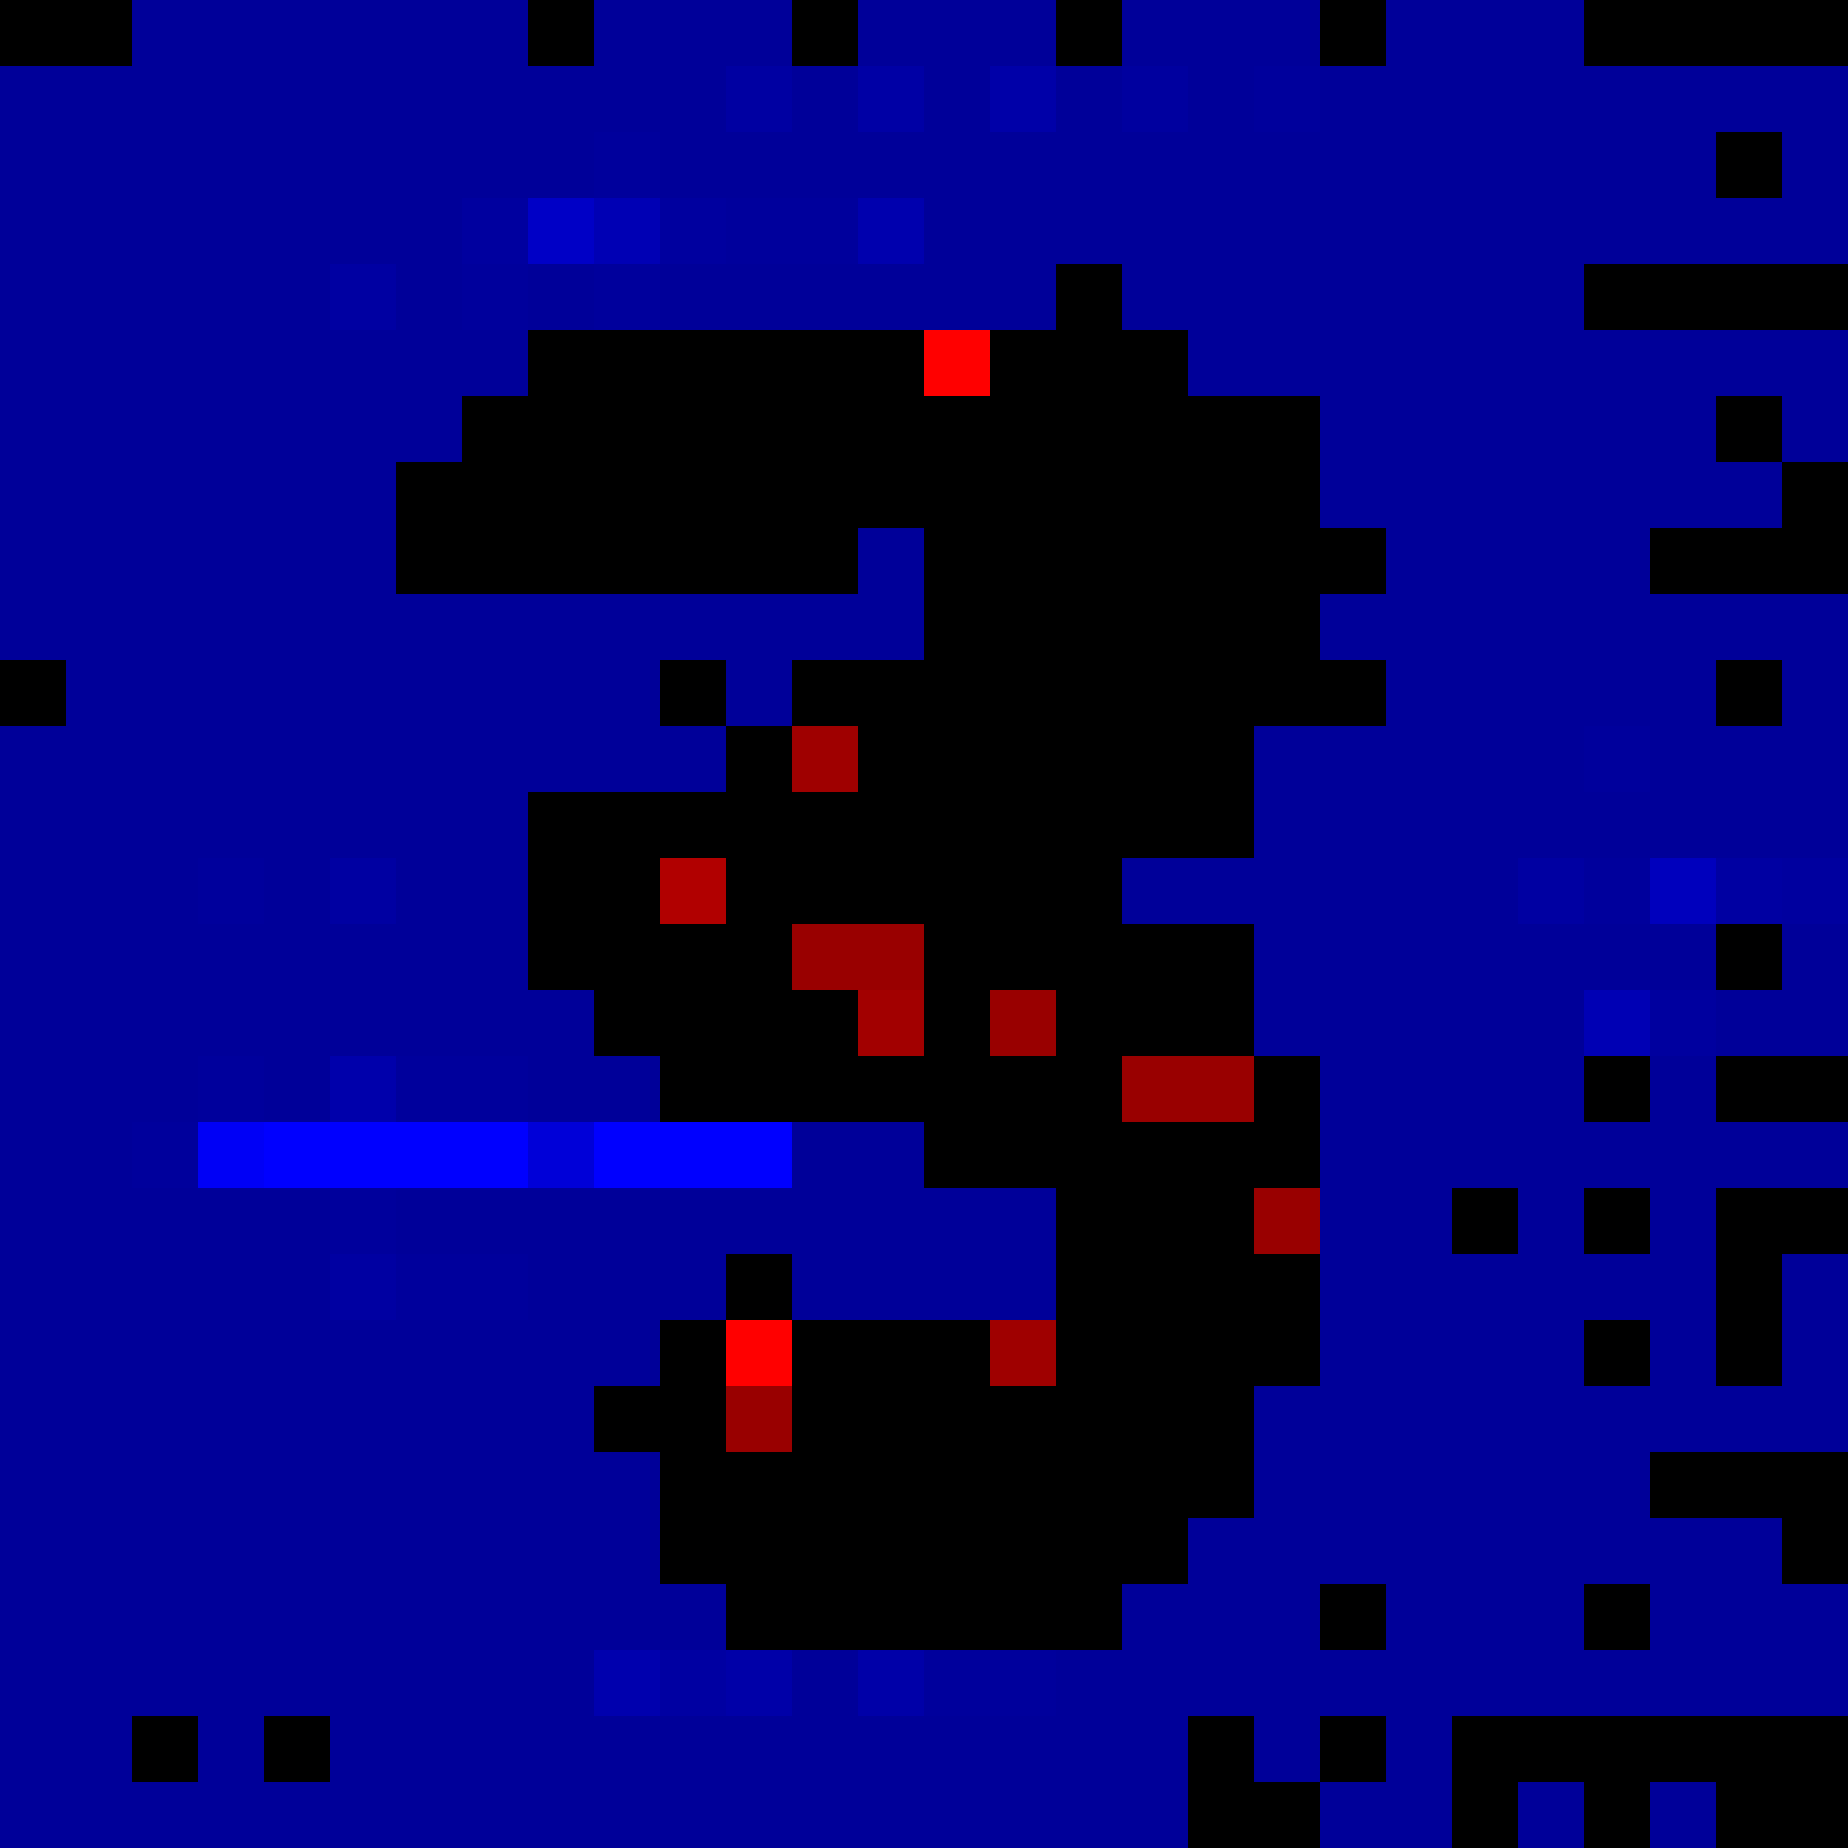
\includegraphics[width=\linewidth]{figures/mnist_split_ic_saliency/image_036_true_3_pred_3/final_saliency_threshold_wrt_6_bright.png}\\[-2pt]{\scriptsize Logit 6}
      \end{minipage}%
      \begin{minipage}[b]{0.19\linewidth}\centering
        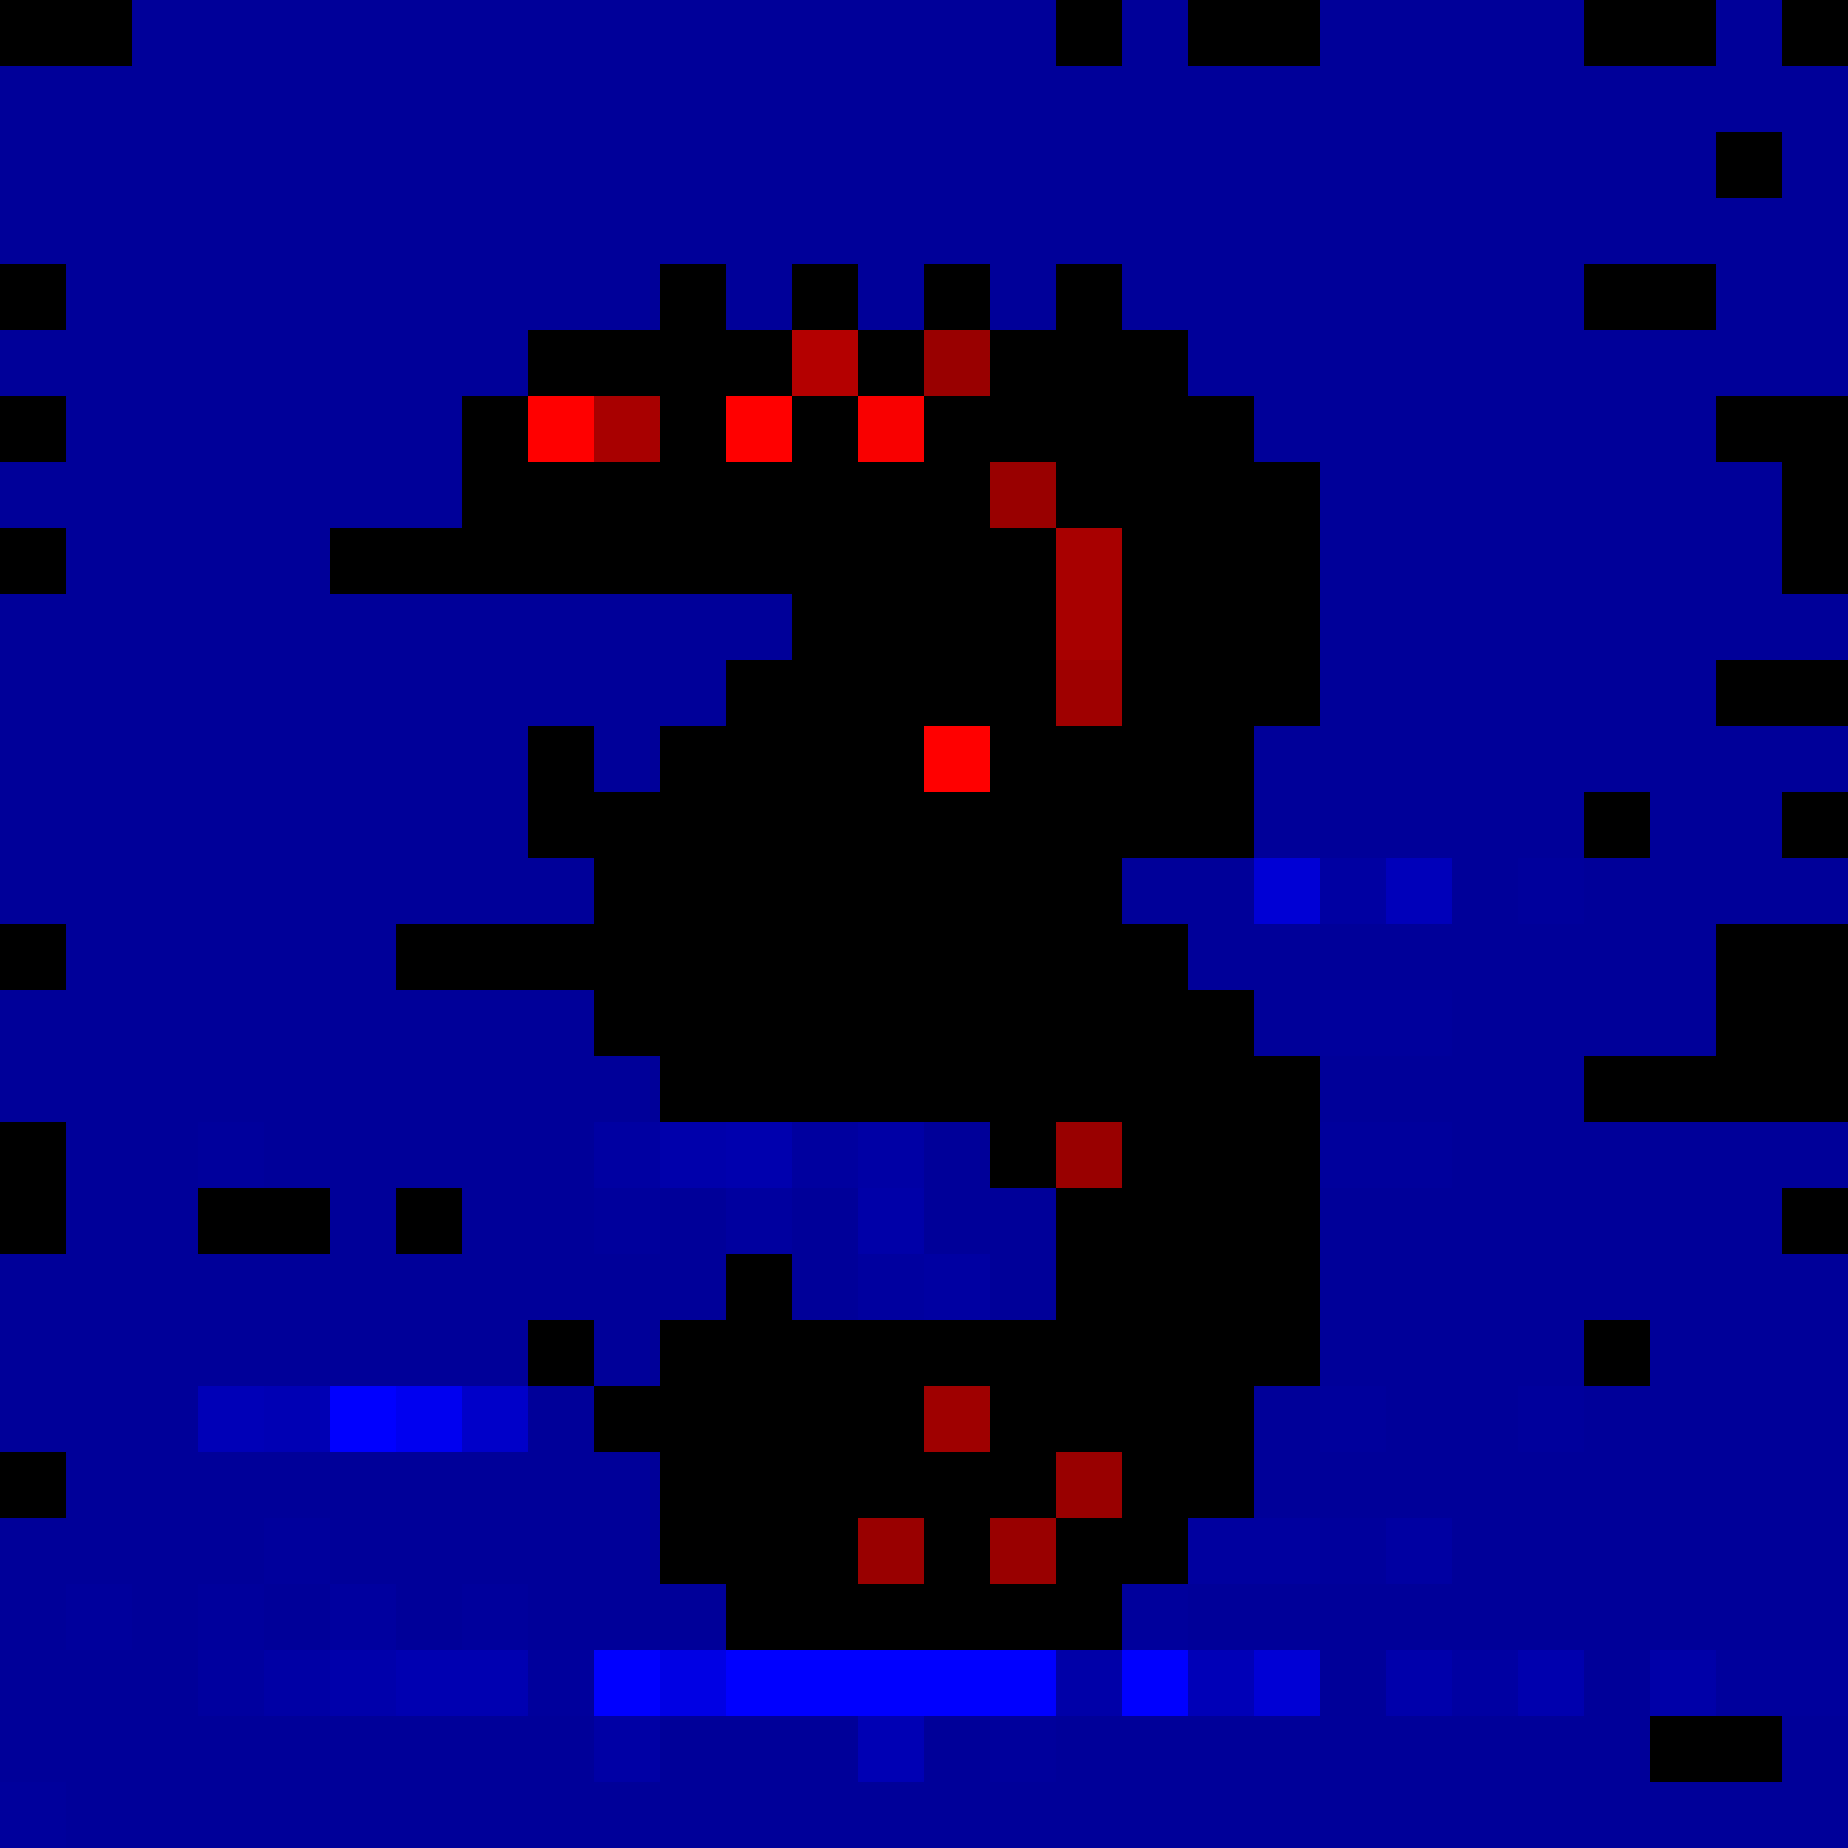
\includegraphics[width=\linewidth]{figures/mnist_split_ic_saliency/image_036_true_3_pred_3/final_saliency_threshold_wrt_7_bright.png}\\[-2pt]{\scriptsize Logit 7}
      \end{minipage}%
      \begin{minipage}[b]{0.19\linewidth}\centering
        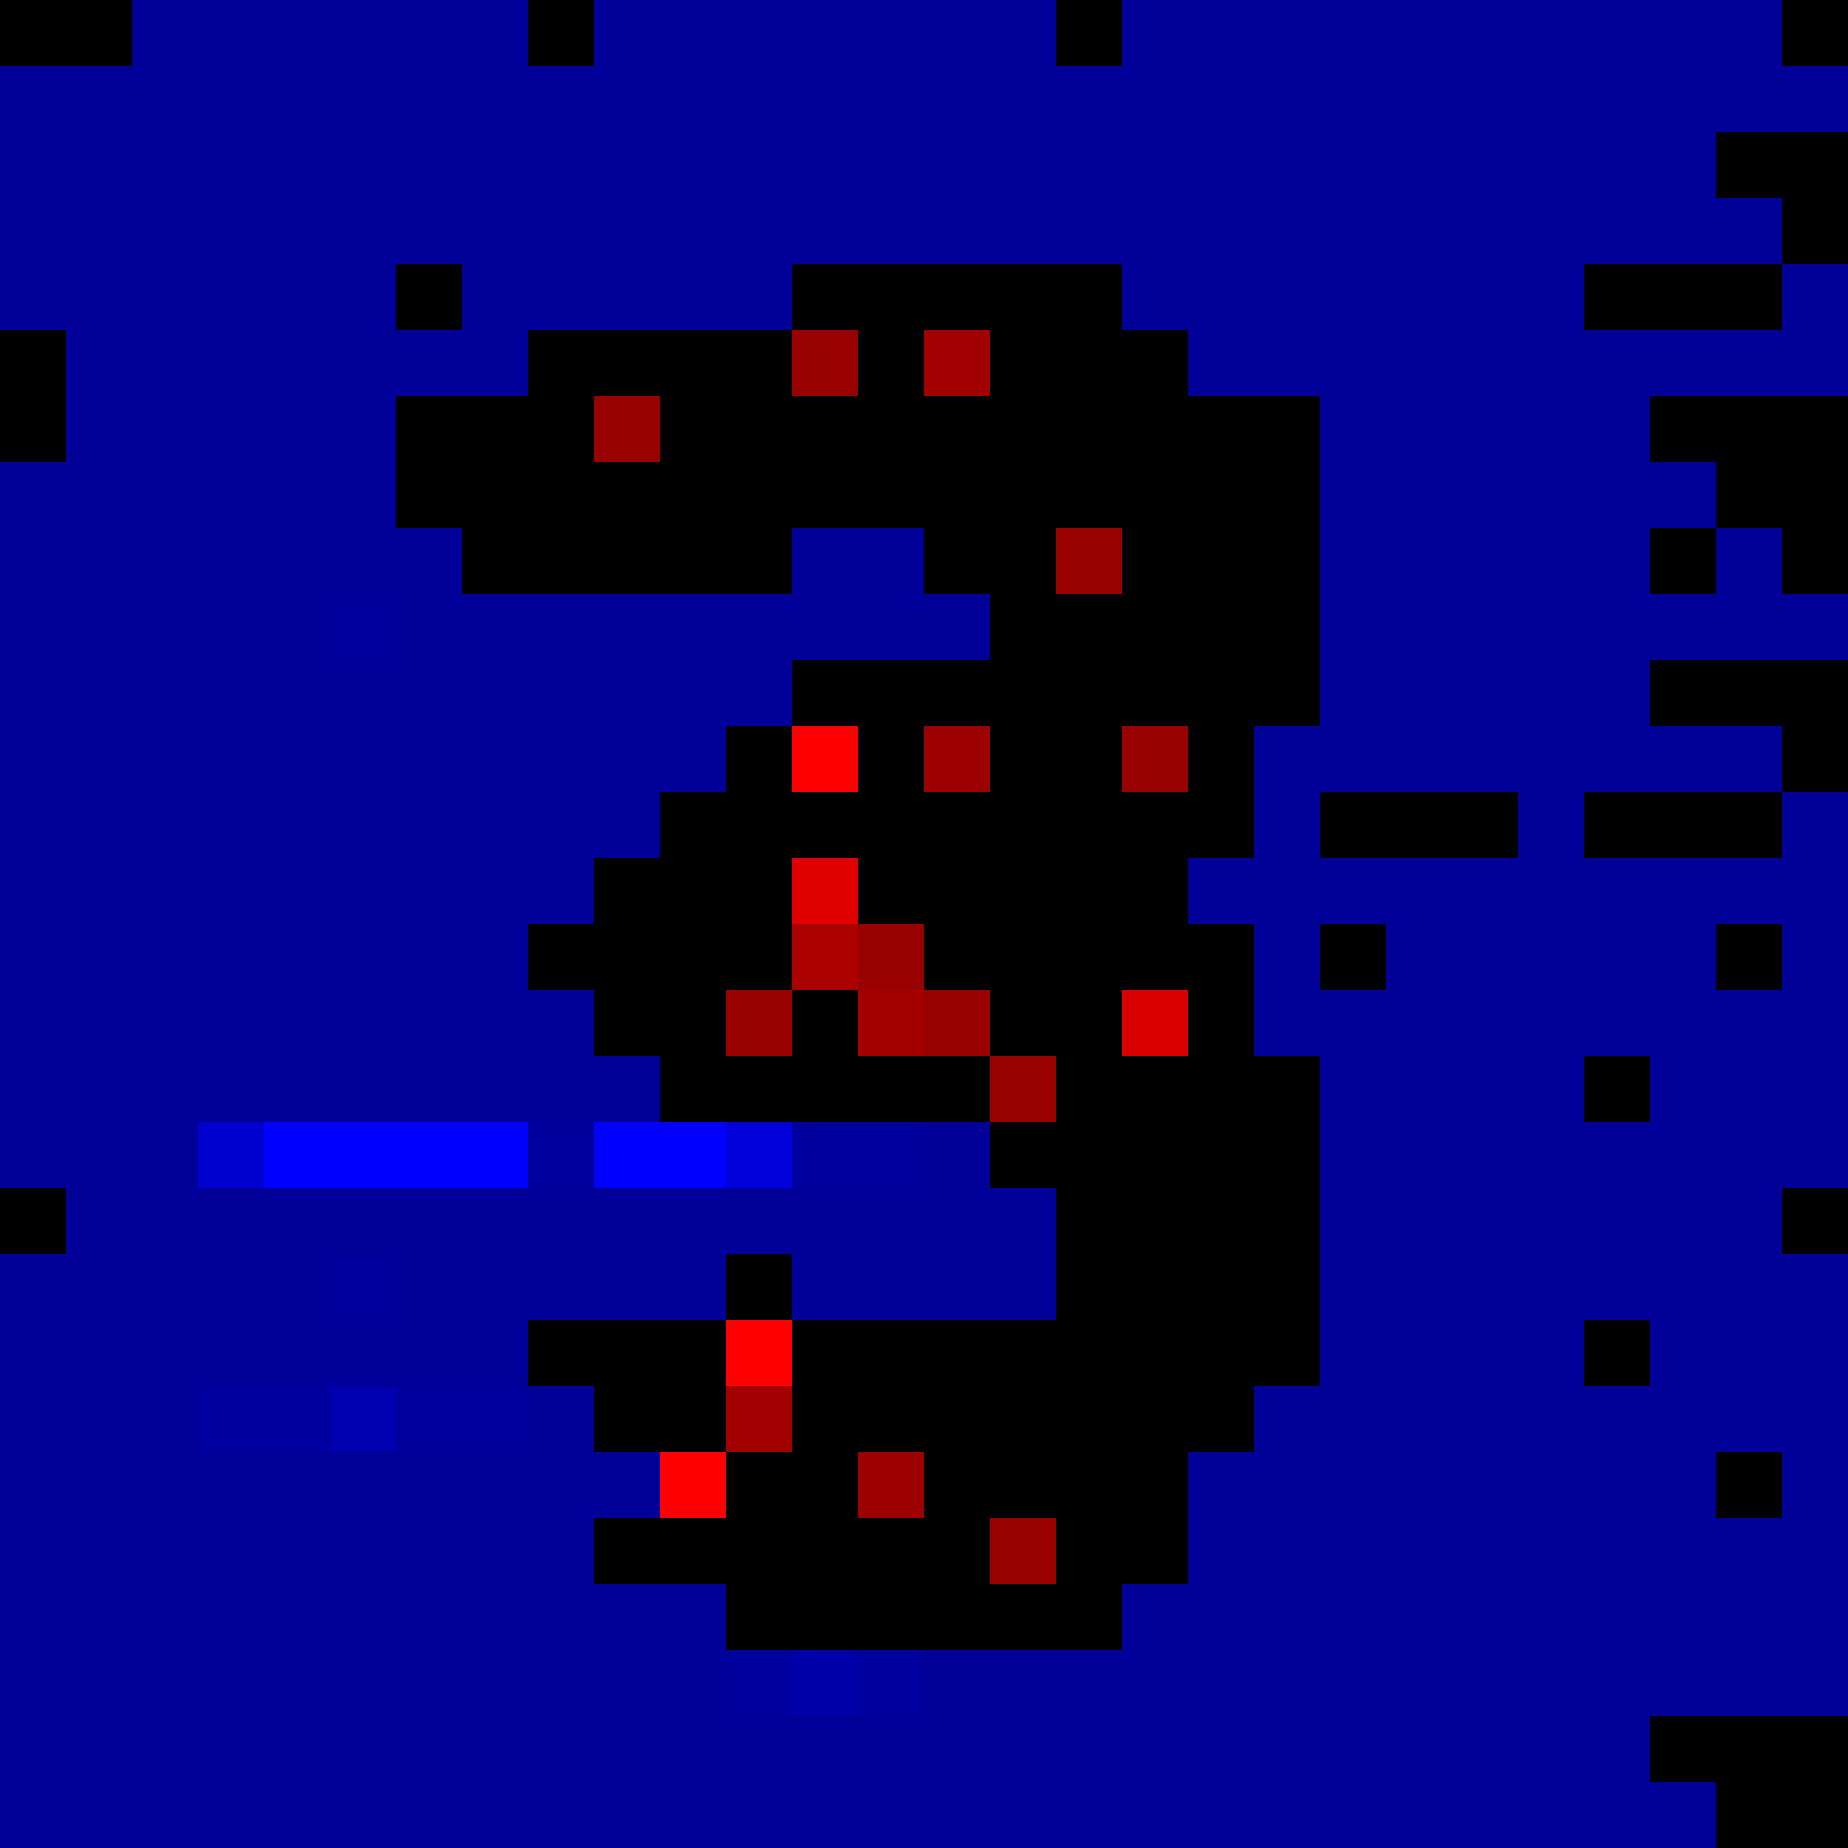
\includegraphics[width=\linewidth]{figures/mnist_split_ic_saliency/image_036_true_3_pred_3/final_saliency_threshold_wrt_8_bright.png}\\[-2pt]{\scriptsize Logit 8}
      \end{minipage}%
      \begin{minipage}[b]{0.19\linewidth}\centering
        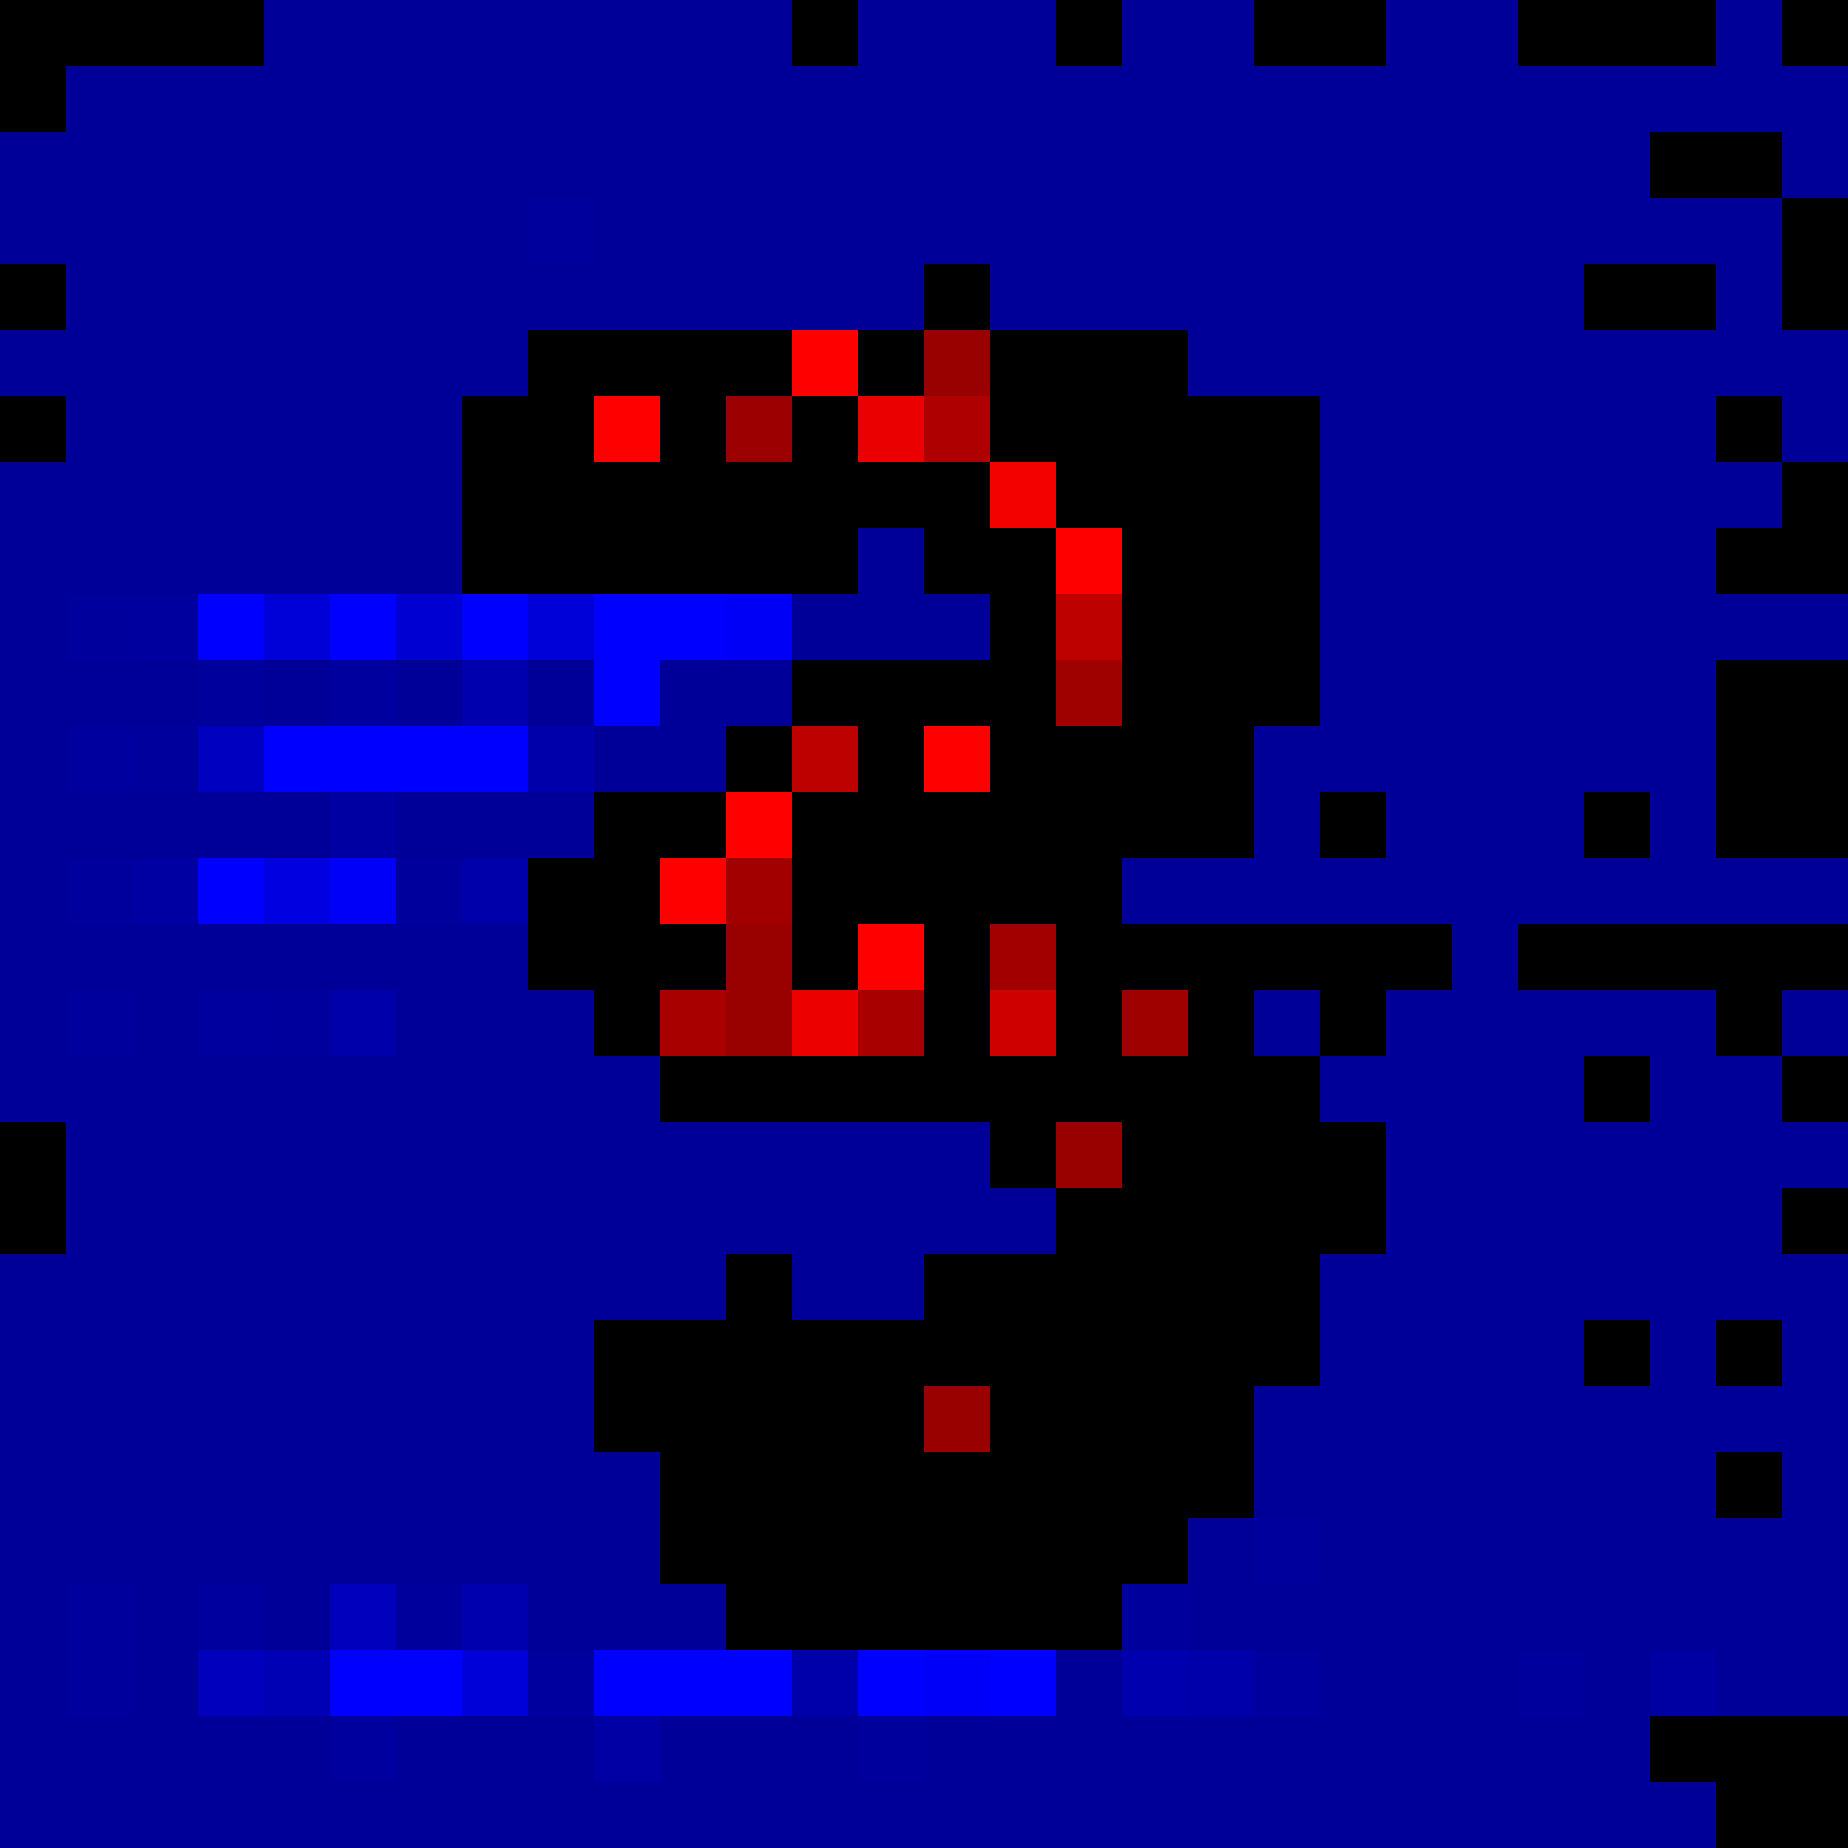
\includegraphics[width=\linewidth]{figures/mnist_split_ic_saliency/image_036_true_3_pred_3/final_saliency_threshold_wrt_9_bright.png}\\[-2pt]{\scriptsize Logit 9}
      \end{minipage}
    \end{minipage}
  
    \caption{Saliency maps for the MNIST Split-IC model. For each example (top: image 030; bottom: image 036), the original digit (left) is shown once, vertically centered beside two rows of five logits (top: 0–4, bottom: 5–9). All tiles are equal size with labels.}
  \end{figure}
  